\chapter{Extended Experimental Results}\label{app:supp_experiments}

The tables and figures below give the complete results for both campaigns. Protocols, metric definitions, validation grids, statistical tests and implementation details appear in Appendix~\ref{app:extended_results}.

\section{Full Evaluation Results for the Split Methods}\label{app:saliency}

This section provides comprehensive evaluation results for all XAI methods tested in the experimental setup described in Section~\ref{sec:experimental_setup}.

\subsection{VGG-16 Qualitative Saliency Map Comparison}\label{app:vgg_qualitative}
Complementing Figure~\ref{fig:vgg_saliency_comparison_main}, we give more saliency examples in Figure~\ref{fig:vgg_saliency_comparison}. Again, we observe more focus on the whole classified objects by SplitCAM in layer 26 compared to LayerCAM in the same layer. SplitGrad in layer 0 detects too many edges of the original image to be a useful explanation of the model's decision, especially with background details such as the rubble in the wood rabbit image. This aligns with the observed performance peaks of SplitGrad and SplitCAM in deeper layers.

\begin{figure}[H]
    \centering

    \begin{minipage}[c]{0.08\linewidth}
        \centering
        \scriptsize \textbf{Class}
    \end{minipage}\hspace{0.002\linewidth}%
    \begin{minipage}[c]{0.10\linewidth}
        \centering
        \scriptsize \textbf{Original}
    \end{minipage}\hspace{0.002\linewidth}%
    \begin{minipage}[c]{0.10\linewidth}
        \centering
        \scriptsize \textbf{SplitLRP}\\
        \scriptsize \textbf{(10, pos) abs}
    \end{minipage}\hspace{0.002\linewidth}%
    \begin{minipage}[c]{0.10\linewidth}
        \centering
        \scriptsize \textbf{LRP $\gamma$=0.25}\\
        \scriptsize \textbf{layer 5 abs}
    \end{minipage}\hspace{0.002\linewidth}%
    \begin{minipage}[c]{0.10\linewidth}
        \centering
        \scriptsize \textbf{SplitCAM}\\
        \scriptsize \textbf{(14, g) $\alpha=0.4$}
    \end{minipage}\hspace{0.002\linewidth}%
    \begin{minipage}[c]{0.10\linewidth}
        \centering
        \scriptsize \textbf{LayerCAM}\\
        \scriptsize \textbf{layer 14}
    \end{minipage}\hspace{0.002\linewidth}%
    \begin{minipage}[c]{0.10\linewidth}
        \centering
        \scriptsize \textbf{SplitCAM}\\
        \scriptsize \textbf{(26, g) $\alpha=0.3$ abs}
    \end{minipage}\hspace{0.002\linewidth}%
    \begin{minipage}[c]{0.10\linewidth}
        \centering
        \scriptsize \textbf{LayerCAM}\\
        \scriptsize \textbf{layer 26}
    \end{minipage}\hspace{0.002\linewidth}%
    \begin{minipage}[c]{0.10\linewidth}
        \centering
        \scriptsize \textbf{SplitGrad}\\
        \scriptsize \textbf{(0, +, g)}
    \end{minipage}

    \vspace{0.3cm}

    \begin{minipage}[c]{0.08\linewidth}
        \centering
        \small tiger shark\\[1pt]
        {\scriptsize (0.9979)}
    \end{minipage}\hspace{0.002\linewidth}%
    \begin{minipage}[c]{0.10\linewidth}
        \centering
        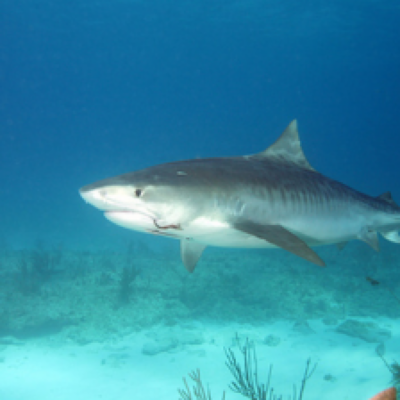
\includegraphics[width=\linewidth]{figures/experiments/saliency_quality/image_0018_ILSVRC2012_val_00034038.JPEG/original_image.png}
    \end{minipage}\hspace{0.002\linewidth}%
    \begin{minipage}[c]{0.10\linewidth}
        \centering
        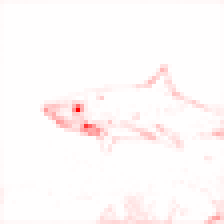
\includegraphics[width=\linewidth]{figures/experiments/saliency_quality/image_0018_ILSVRC2012_val_00034038.JPEG/hybrid_lrp_scaling_max_winnerTakesItAllMaxpool_f10_cam_pp_abs.png}
    \end{minipage}\hspace{0.002\linewidth}%
    \begin{minipage}[c]{0.10\linewidth}
        \centering
        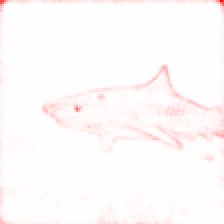
\includegraphics[width=\linewidth]{figures/experiments/saliency_quality/image_0018_ILSVRC2012_val_00034038.JPEG/zennit_lrp_gamma0.25_features_5_abs.png}
    \end{minipage}\hspace{0.002\linewidth}%
    \begin{minipage}[c]{0.10\linewidth}
        \centering
        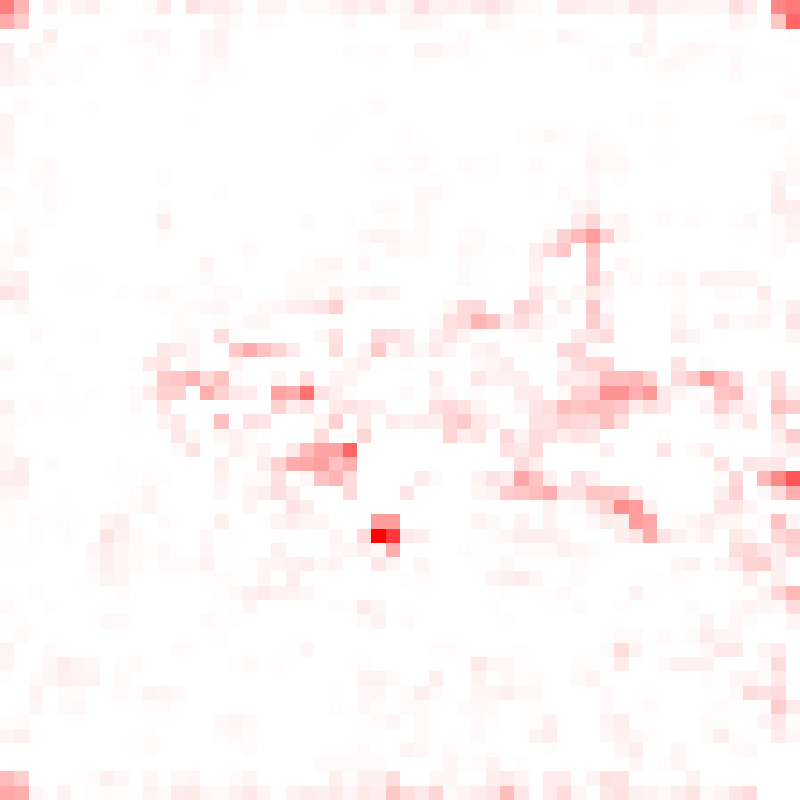
\includegraphics[width=\linewidth]{figures/experiments/saliency_quality/image_0018_ILSVRC2012_val_00034038.JPEG/hybrid_cam_shift_40_scale_max_winnerTakesItAllMaxpool_f14_cam_g.png}
    \end{minipage}\hspace{0.002\linewidth}%
    \begin{minipage}[c]{0.10\linewidth}
        \centering
        
\includegraphics[width=\linewidth]{figures/experiments/saliency_quality/image_0018_ILSVRC2012_val_00034038.JPEG/layer_cam_features_14_relu.png}
    \end{minipage}\hspace{0.002\linewidth}%
    \begin{minipage}[c]{0.10\linewidth}
        \centering
        
\includegraphics[width=\linewidth]{figures/experiments/saliency_quality/image_0018_ILSVRC2012_val_00034038.JPEG/hybrid_cam_shift_30_scale_max_winnerTakesItAllMaxpool_f26_cam_g_abs.png}
    \end{minipage}\hspace{0.002\linewidth}%
    \begin{minipage}[c]{0.10\linewidth}
        \centering
        
\includegraphics[width=\linewidth]{figures/experiments/saliency_quality/image_0018_ILSVRC2012_val_00034038.JPEG/layer_cam_features_26_relu.png}
    \end{minipage}\hspace{0.002\linewidth}%
    \begin{minipage}[c]{0.10\linewidth}
        \centering
        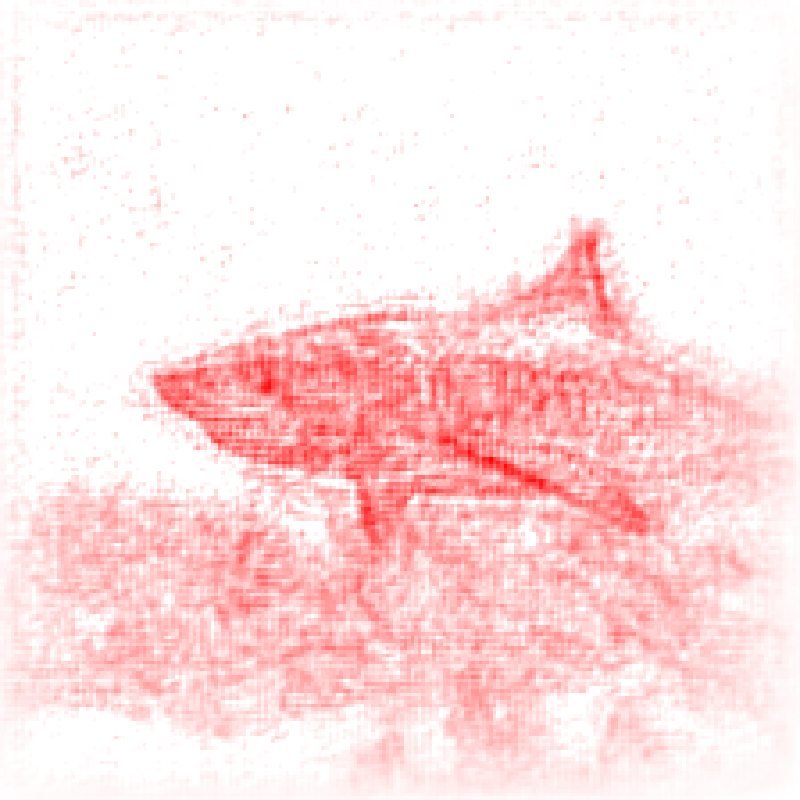
\includegraphics[width=\linewidth]{figures/experiments/saliency_quality/image_0018_ILSVRC2012_val_00034038.JPEG/hybrid_grad_shift_30_max_winnerTakesItAllMaxpool_f0_grad_pp.png}
    \end{minipage}%

    \vspace{0.3cm}

    \begin{minipage}[c]{0.08\linewidth}
        \centering
        \small goldfinch\\[1pt]
        {\scriptsize (1.0000)}
    \end{minipage}\hspace{0.002\linewidth}%
    \begin{minipage}[c]{0.10\linewidth}
        \centering
        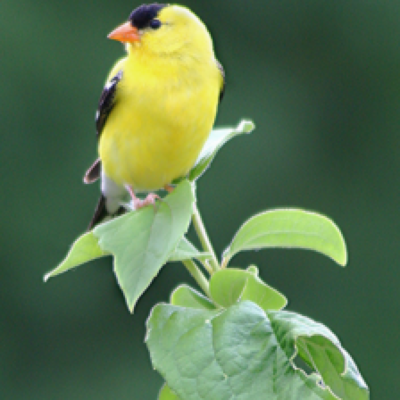
\includegraphics[width=\linewidth]{figures/experiments/saliency_quality/image_0034_ILSVRC2012_val_00044706.JPEG/original_image.png}
    \end{minipage}\hspace{0.002\linewidth}%
    \begin{minipage}[c]{0.10\linewidth}
        \centering
        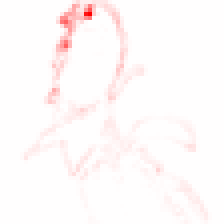
\includegraphics[width=\linewidth]{figures/experiments/saliency_quality/image_0034_ILSVRC2012_val_00044706.JPEG/hybrid_lrp_scaling_max_winnerTakesItAllMaxpool_f10_cam_pp_abs.png}
    \end{minipage}\hspace{0.002\linewidth}%
    \begin{minipage}[c]{0.10\linewidth}
        \centering
        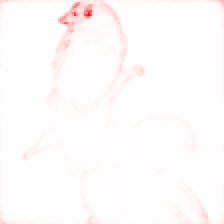
\includegraphics[width=\linewidth]{figures/experiments/saliency_quality/image_0034_ILSVRC2012_val_00044706.JPEG/zennit_lrp_gamma0.25_features_5_abs.png}
    \end{minipage}\hspace{0.002\linewidth}%
    \begin{minipage}[c]{0.10\linewidth}
        \centering
        
\includegraphics[width=\linewidth]{figures/experiments/saliency_quality/image_0034_ILSVRC2012_val_00044706.JPEG/hybrid_cam_shift_40_scale_max_winnerTakesItAllMaxpool_f14_cam_g.png}
    \end{minipage}\hspace{0.002\linewidth}%
    \begin{minipage}[c]{0.10\linewidth}
        \centering
        
\includegraphics[width=\linewidth]{figures/experiments/saliency_quality/image_0034_ILSVRC2012_val_00044706.JPEG/layer_cam_features_14_relu.png}
    \end{minipage}\hspace{0.002\linewidth}%
    \begin{minipage}[c]{0.10\linewidth}
        \centering
        
\includegraphics[width=\linewidth]{figures/experiments/saliency_quality/image_0034_ILSVRC2012_val_00044706.JPEG/hybrid_cam_shift_30_scale_max_winnerTakesItAllMaxpool_f26_cam_g_abs.png}
    \end{minipage}\hspace{0.002\linewidth}%
    \begin{minipage}[c]{0.10\linewidth}
        \centering
        
\includegraphics[width=\linewidth]{figures/experiments/saliency_quality/image_0034_ILSVRC2012_val_00044706.JPEG/layer_cam_features_26_relu.png}
    \end{minipage}\hspace{0.002\linewidth}%
    \begin{minipage}[c]{0.10\linewidth}
        \centering
        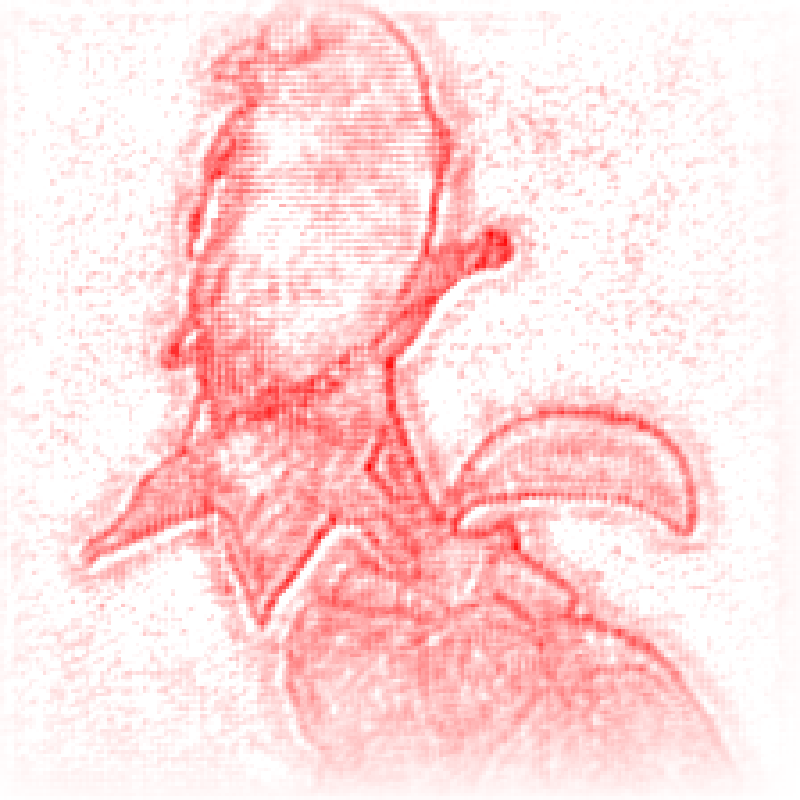
\includegraphics[width=\linewidth]{figures/experiments/saliency_quality/image_0034_ILSVRC2012_val_00044706.JPEG/hybrid_grad_shift_30_max_winnerTakesItAllMaxpool_f0_grad_pp.png}
    \end{minipage}%

    \vspace{0.3cm}

    \begin{minipage}[c]{0.08\linewidth}
        \centering
        \small tree frog\\[1pt]
        {\scriptsize (0.9954)}
    \end{minipage}\hspace{0.002\linewidth}%
    \begin{minipage}[c]{0.10\linewidth}
        \centering
        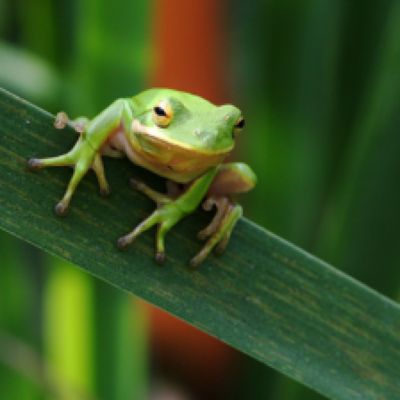
\includegraphics[width=\linewidth]{figures/experiments/saliency_quality/image_0041_ILSVRC2012_val_00017505.JPEG/original_image.png}
    \end{minipage}\hspace{0.002\linewidth}%
    \begin{minipage}[c]{0.10\linewidth}
        \centering
        
\includegraphics[width=\linewidth]{figures/experiments/saliency_quality/image_0041_ILSVRC2012_val_00017505.JPEG/hybrid_lrp_scaling_max_winnerTakesItAllMaxpool_f10_cam_pp_abs.png}
    \end{minipage}\hspace{0.002\linewidth}%
    \begin{minipage}[c]{0.10\linewidth}
        \centering
        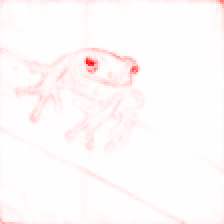
\includegraphics[width=\linewidth]{figures/experiments/saliency_quality/image_0041_ILSVRC2012_val_00017505.JPEG/zennit_lrp_gamma0.25_features_5_abs.png}
    \end{minipage}\hspace{0.002\linewidth}%
    \begin{minipage}[c]{0.10\linewidth}
        \centering
        
\includegraphics[width=\linewidth]{figures/experiments/saliency_quality/image_0041_ILSVRC2012_val_00017505.JPEG/hybrid_cam_shift_40_scale_max_winnerTakesItAllMaxpool_f14_cam_g.png}
    \end{minipage}\hspace{0.002\linewidth}%
    \begin{minipage}[c]{0.10\linewidth}
        \centering
        
\includegraphics[width=\linewidth]{figures/experiments/saliency_quality/image_0041_ILSVRC2012_val_00017505.JPEG/layer_cam_features_14_relu.png}
    \end{minipage}\hspace{0.002\linewidth}%
    \begin{minipage}[c]{0.10\linewidth}
        \centering
        
\includegraphics[width=\linewidth]{figures/experiments/saliency_quality/image_0041_ILSVRC2012_val_00017505.JPEG/hybrid_cam_shift_30_scale_max_winnerTakesItAllMaxpool_f26_cam_g_abs.png}
    \end{minipage}\hspace{0.002\linewidth}%
    \begin{minipage}[c]{0.10\linewidth}
        \centering
        
\includegraphics[width=\linewidth]{figures/experiments/saliency_quality/image_0041_ILSVRC2012_val_00017505.JPEG/layer_cam_features_26_relu.png}
    \end{minipage}\hspace{0.002\linewidth}%
    \begin{minipage}[c]{0.10\linewidth}
        \centering
        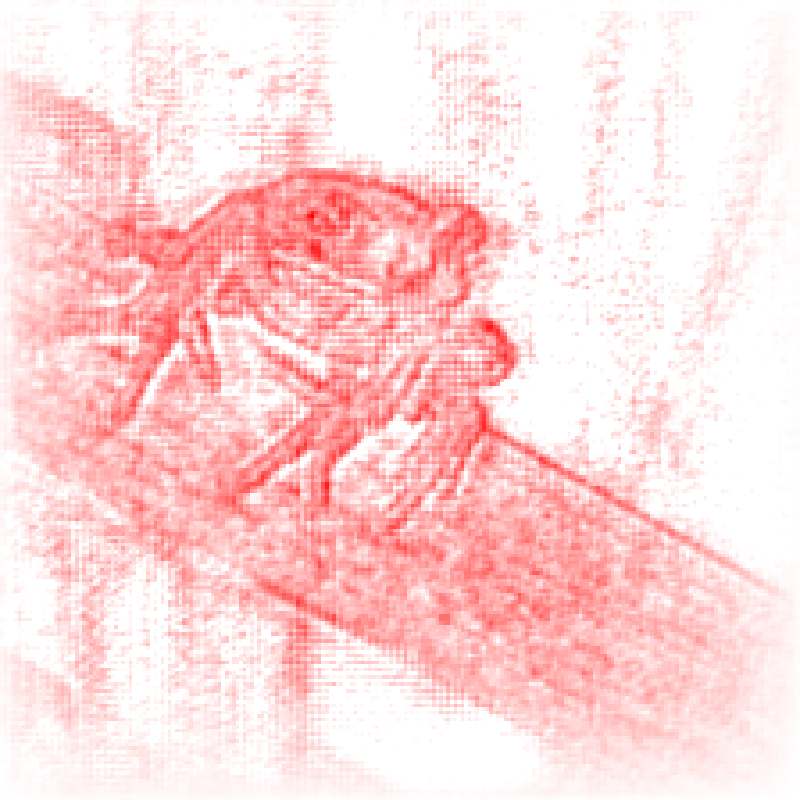
\includegraphics[width=\linewidth]{figures/experiments/saliency_quality/image_0041_ILSVRC2012_val_00017505.JPEG/hybrid_grad_shift_30_max_winnerTakesItAllMaxpool_f0_grad_pp.png}
    \end{minipage}%

    \vspace{0.3cm}

    \begin{minipage}[c]{0.08\linewidth}
        \centering
        \small ladybug\\[1pt]
        {\scriptsize (0.8272)}
    \end{minipage}\hspace{0.002\linewidth}%
    \begin{minipage}[c]{0.10\linewidth}
        \centering
        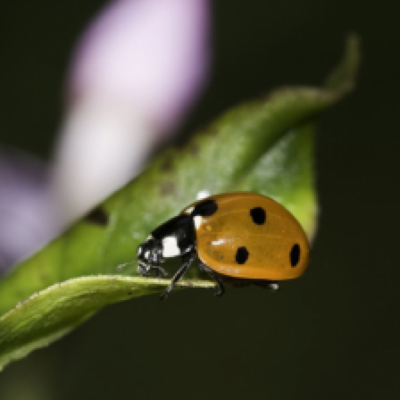
\includegraphics[width=\linewidth]{figures/experiments/saliency_quality/image_0096_ILSVRC2012_val_00025218.JPEG/original_image.png}
    \end{minipage}\hspace{0.002\linewidth}%
    \begin{minipage}[c]{0.10\linewidth}
        \centering
        
\includegraphics[width=\linewidth]{figures/experiments/saliency_quality/image_0096_ILSVRC2012_val_00025218.JPEG/hybrid_lrp_scaling_max_winnerTakesItAllMaxpool_f10_cam_pp_abs.png}
    \end{minipage}\hspace{0.002\linewidth}%
    \begin{minipage}[c]{0.10\linewidth}
        \centering
        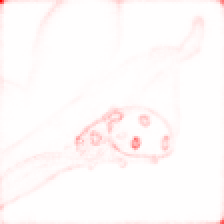
\includegraphics[width=\linewidth]{figures/experiments/saliency_quality/image_0096_ILSVRC2012_val_00025218.JPEG/zennit_lrp_gamma0.25_features_5_abs.png}
    \end{minipage}\hspace{0.002\linewidth}%
    \begin{minipage}[c]{0.10\linewidth}
        \centering
        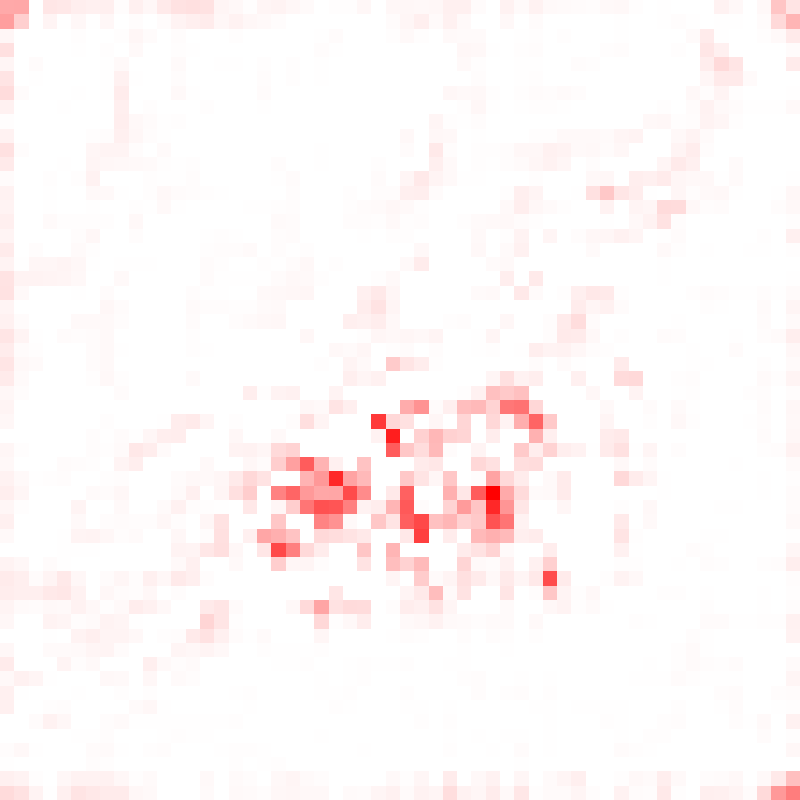
\includegraphics[width=\linewidth]{figures/experiments/saliency_quality/image_0096_ILSVRC2012_val_00025218.JPEG/hybrid_cam_shift_40_scale_max_winnerTakesItAllMaxpool_f14_cam_g.png}
    \end{minipage}\hspace{0.002\linewidth}%
    \begin{minipage}[c]{0.10\linewidth}
        \centering
        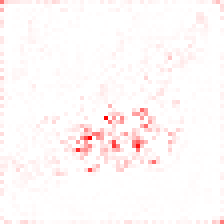
\includegraphics[width=\linewidth]{figures/experiments/saliency_quality/image_0096_ILSVRC2012_val_00025218.JPEG/layer_cam_features_14_relu.png}
    \end{minipage}\hspace{0.002\linewidth}%
    \begin{minipage}[c]{0.10\linewidth}
        \centering
        
\includegraphics[width=\linewidth]{figures/experiments/saliency_quality/image_0096_ILSVRC2012_val_00025218.JPEG/hybrid_cam_shift_30_scale_max_winnerTakesItAllMaxpool_f26_cam_g_abs.png}
    \end{minipage}\hspace{0.002\linewidth}%
    \begin{minipage}[c]{0.10\linewidth}
        \centering
        
\includegraphics[width=\linewidth]{figures/experiments/saliency_quality/image_0096_ILSVRC2012_val_00025218.JPEG/layer_cam_features_26_relu.png}
    \end{minipage}\hspace{0.002\linewidth}%
    \begin{minipage}[c]{0.10\linewidth}
        \centering
        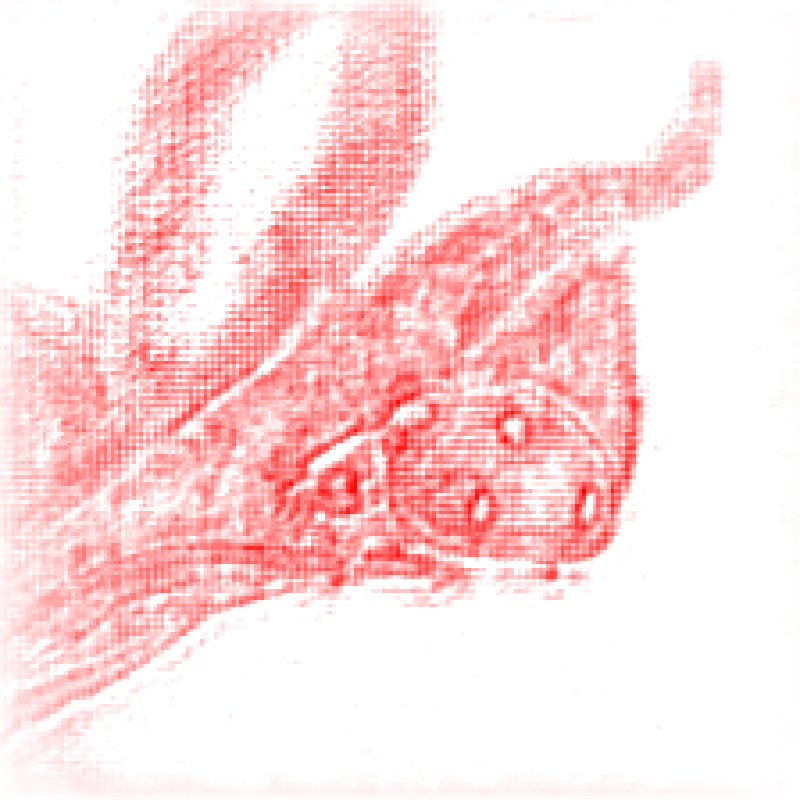
\includegraphics[width=\linewidth]{figures/experiments/saliency_quality/image_0096_ILSVRC2012_val_00025218.JPEG/hybrid_grad_shift_30_max_winnerTakesItAllMaxpool_f0_grad_pp.png}
    \end{minipage}%

    \vspace{0.3cm}

    \begin{minipage}[c]{0.08\linewidth}
        \centering
        \small wood rabbit\\[1pt]
        {\scriptsize (0.9782)}
    \end{minipage}\hspace{0.002\linewidth}%
    \begin{minipage}[c]{0.10\linewidth}
        \centering
        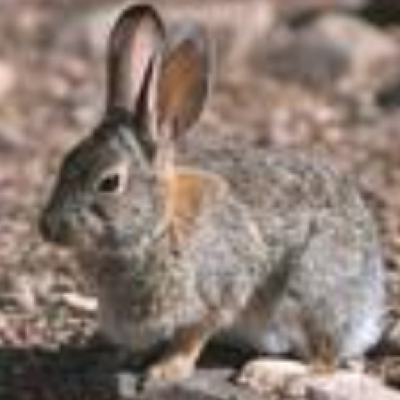
\includegraphics[width=\linewidth]{figures/experiments/saliency_quality/image_0120_ILSVRC2012_val_00024858.JPEG/original_image.png}
    \end{minipage}\hspace{0.002\linewidth}%
    \begin{minipage}[c]{0.10\linewidth}
        \centering
        
\includegraphics[width=\linewidth]{figures/experiments/saliency_quality/image_0120_ILSVRC2012_val_00024858.JPEG/hybrid_lrp_scaling_max_winnerTakesItAllMaxpool_f10_cam_pp_abs.png}
    \end{minipage}\hspace{0.002\linewidth}%
    \begin{minipage}[c]{0.10\linewidth}
        \centering
        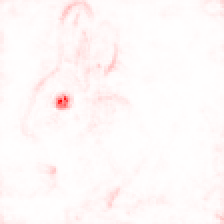
\includegraphics[width=\linewidth]{figures/experiments/saliency_quality/image_0120_ILSVRC2012_val_00024858.JPEG/zennit_lrp_gamma0.25_features_5_abs.png}
    \end{minipage}\hspace{0.002\linewidth}%
    \begin{minipage}[c]{0.10\linewidth}
        \centering
        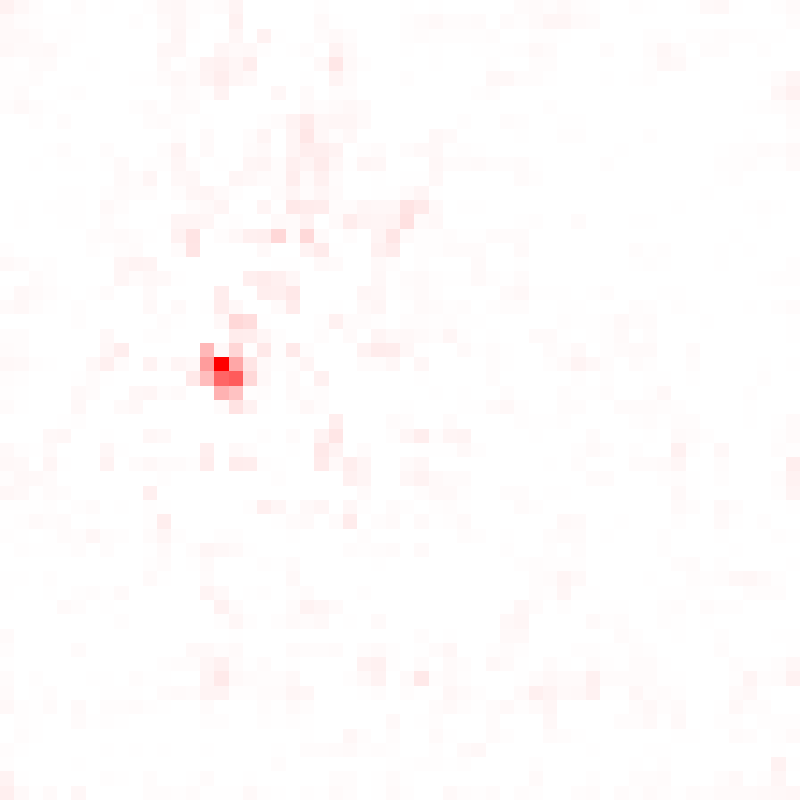
\includegraphics[width=\linewidth]{figures/experiments/saliency_quality/image_0120_ILSVRC2012_val_00024858.JPEG/hybrid_cam_shift_40_scale_max_winnerTakesItAllMaxpool_f14_cam_g.png}
    \end{minipage}\hspace{0.002\linewidth}%
    \begin{minipage}[c]{0.10\linewidth}
        \centering
        
\includegraphics[width=\linewidth]{figures/experiments/saliency_quality/image_0120_ILSVRC2012_val_00024858.JPEG/layer_cam_features_14_relu.png}
    \end{minipage}\hspace{0.002\linewidth}%
    \begin{minipage}[c]{0.10\linewidth}
        \centering
        
\includegraphics[width=\linewidth]{figures/experiments/saliency_quality/image_0120_ILSVRC2012_val_00024858.JPEG/hybrid_cam_shift_30_scale_max_winnerTakesItAllMaxpool_f26_cam_g_abs.png}
    \end{minipage}\hspace{0.002\linewidth}%
    \begin{minipage}[c]{0.10\linewidth}
        \centering
        
\includegraphics[width=\linewidth]{figures/experiments/saliency_quality/image_0120_ILSVRC2012_val_00024858.JPEG/layer_cam_features_26_relu.png}
    \end{minipage}\hspace{0.002\linewidth}%
    \begin{minipage}[c]{0.10\linewidth}
        \centering
        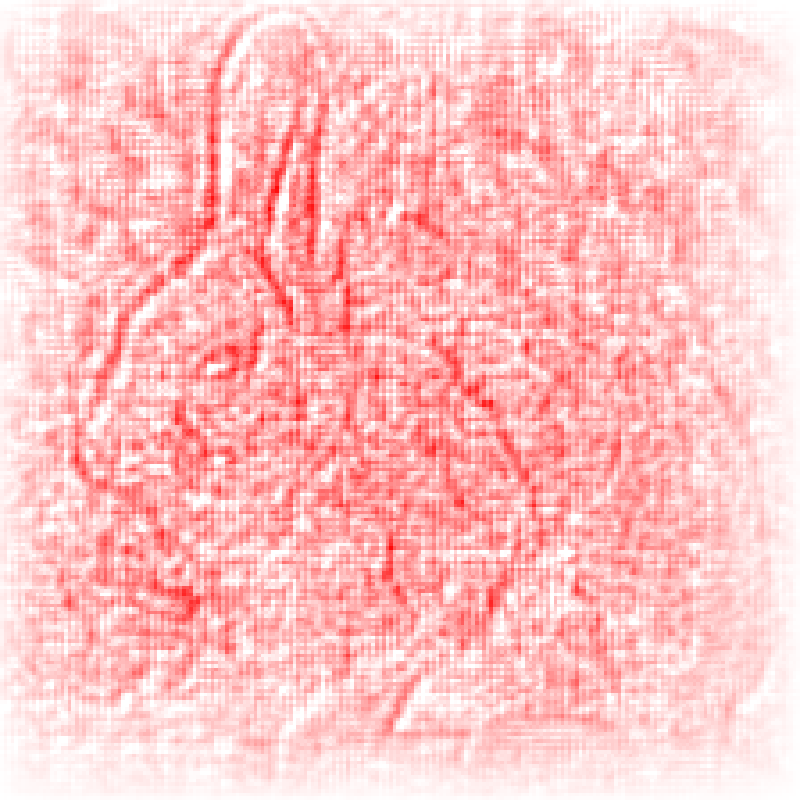
\includegraphics[width=\linewidth]{figures/experiments/saliency_quality/image_0120_ILSVRC2012_val_00024858.JPEG/hybrid_grad_shift_30_max_winnerTakesItAllMaxpool_f0_grad_pp.png}
    \end{minipage}%

    \vspace{0.3cm}

    \begin{minipage}[c]{0.08\linewidth}
        \centering
        \small water tower\\[1pt]
        {\scriptsize (1.0000)}
    \end{minipage}\hspace{0.002\linewidth}%
    \begin{minipage}[c]{0.10\linewidth}
        \centering
        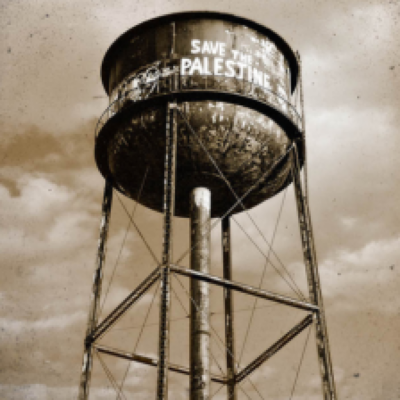
\includegraphics[width=\linewidth]{figures/experiments/saliency_quality/image_0499_ILSVRC2012_val_00037082.JPEG/original_image.png}
    \end{minipage}\hspace{0.002\linewidth}%
    \begin{minipage}[c]{0.10\linewidth}
        \centering
        
\includegraphics[width=\linewidth]{figures/experiments/saliency_quality/image_0499_ILSVRC2012_val_00037082.JPEG/hybrid_lrp_scaling_max_winnerTakesItAllMaxpool_f10_cam_pp_abs.png}
    \end{minipage}\hspace{0.002\linewidth}%
    \begin{minipage}[c]{0.10\linewidth}
        \centering
        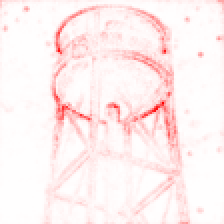
\includegraphics[width=\linewidth]{figures/experiments/saliency_quality/image_0499_ILSVRC2012_val_00037082.JPEG/zennit_lrp_gamma0.25_features_5_abs.png}
    \end{minipage}\hspace{0.002\linewidth}%
    \begin{minipage}[c]{0.10\linewidth}
        \centering
        
\includegraphics[width=\linewidth]{figures/experiments/saliency_quality/image_0499_ILSVRC2012_val_00037082.JPEG/hybrid_cam_shift_40_scale_max_winnerTakesItAllMaxpool_f14_cam_g.png}
    \end{minipage}\hspace{0.002\linewidth}%
    \begin{minipage}[c]{0.10\linewidth}
        \centering
        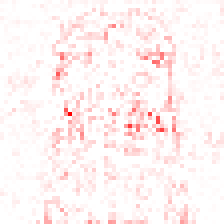
\includegraphics[width=\linewidth]{figures/experiments/saliency_quality/image_0499_ILSVRC2012_val_00037082.JPEG/layer_cam_features_14_relu.png}
    \end{minipage}\hspace{0.002\linewidth}%
    \begin{minipage}[c]{0.10\linewidth}
        \centering
        
\includegraphics[width=\linewidth]{figures/experiments/saliency_quality/image_0499_ILSVRC2012_val_00037082.JPEG/hybrid_cam_shift_30_scale_max_winnerTakesItAllMaxpool_f26_cam_g_abs.png}
    \end{minipage}\hspace{0.002\linewidth}%
    \begin{minipage}[c]{0.10\linewidth}
        \centering
        
\includegraphics[width=\linewidth]{figures/experiments/saliency_quality/image_0499_ILSVRC2012_val_00037082.JPEG/layer_cam_features_26_relu.png}
    \end{minipage}\hspace{0.002\linewidth}%
    \begin{minipage}[c]{0.10\linewidth}
        \centering
        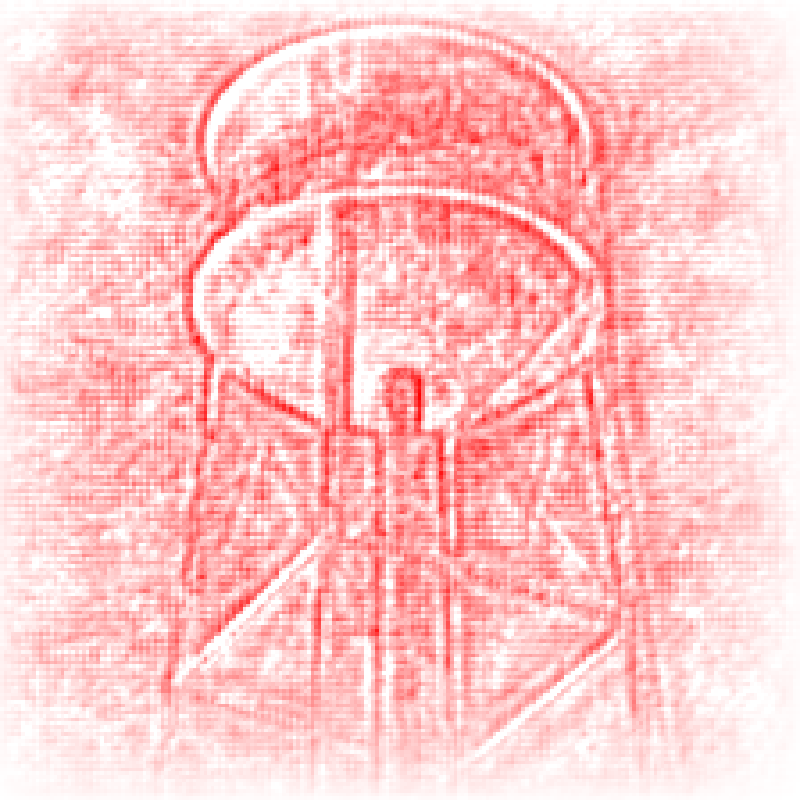
\includegraphics[width=\linewidth]{figures/experiments/saliency_quality/image_0499_ILSVRC2012_val_00037082.JPEG/hybrid_grad_shift_30_max_winnerTakesItAllMaxpool_f0_grad_pp.png}
    \end{minipage}%

    \vspace{0.3cm}

    \begin{minipage}[c]{0.08\linewidth}
        \centering
        \small yawl\\[1pt]
        {\scriptsize (0.9953)}
    \end{minipage}\hspace{0.002\linewidth}%
    \begin{minipage}[c]{0.10\linewidth}
        \centering
        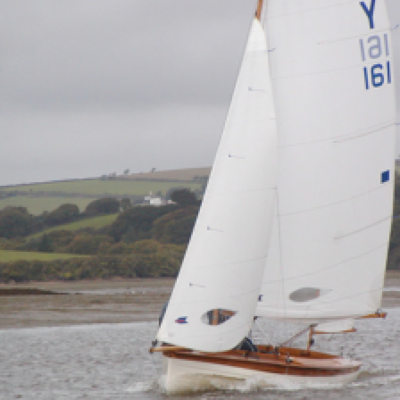
\includegraphics[width=\linewidth]{figures/experiments/saliency_quality/image_0511_ILSVRC2012_val_00035734.JPEG/original_image.png}
    \end{minipage}\hspace{0.002\linewidth}%
    \begin{minipage}[c]{0.10\linewidth}
        \centering
        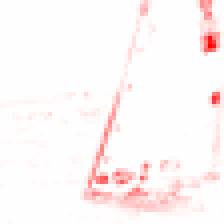
\includegraphics[width=\linewidth]{figures/experiments/saliency_quality/image_0511_ILSVRC2012_val_00035734.JPEG/hybrid_lrp_scaling_max_winnerTakesItAllMaxpool_f10_cam_pp_abs.png}
    \end{minipage}\hspace{0.002\linewidth}%
    \begin{minipage}[c]{0.10\linewidth}
        \centering
        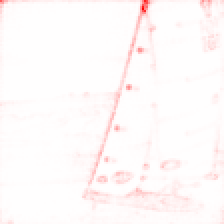
\includegraphics[width=\linewidth]{figures/experiments/saliency_quality/image_0511_ILSVRC2012_val_00035734.JPEG/zennit_lrp_gamma0.25_features_5_abs.png}
    \end{minipage}\hspace{0.002\linewidth}%
    \begin{minipage}[c]{0.10\linewidth}
        \centering
        
\includegraphics[width=\linewidth]{figures/experiments/saliency_quality/image_0511_ILSVRC2012_val_00035734.JPEG/hybrid_cam_shift_40_scale_max_winnerTakesItAllMaxpool_f14_cam_g.png}
    \end{minipage}\hspace{0.002\linewidth}%
    \begin{minipage}[c]{0.10\linewidth}
        \centering
        
\includegraphics[width=\linewidth]{figures/experiments/saliency_quality/image_0511_ILSVRC2012_val_00035734.JPEG/layer_cam_features_14_relu.png}
    \end{minipage}\hspace{0.002\linewidth}%
    \begin{minipage}[c]{0.10\linewidth}
        \centering
        
\includegraphics[width=\linewidth]{figures/experiments/saliency_quality/image_0511_ILSVRC2012_val_00035734.JPEG/hybrid_cam_shift_30_scale_max_winnerTakesItAllMaxpool_f26_cam_g_abs.png}
    \end{minipage}\hspace{0.002\linewidth}%
    \begin{minipage}[c]{0.10\linewidth}
        \centering
        
\includegraphics[width=\linewidth]{figures/experiments/saliency_quality/image_0511_ILSVRC2012_val_00035734.JPEG/layer_cam_features_26_relu.png}
    \end{minipage}\hspace{0.002\linewidth}%
    \begin{minipage}[c]{0.10\linewidth}
        \centering
        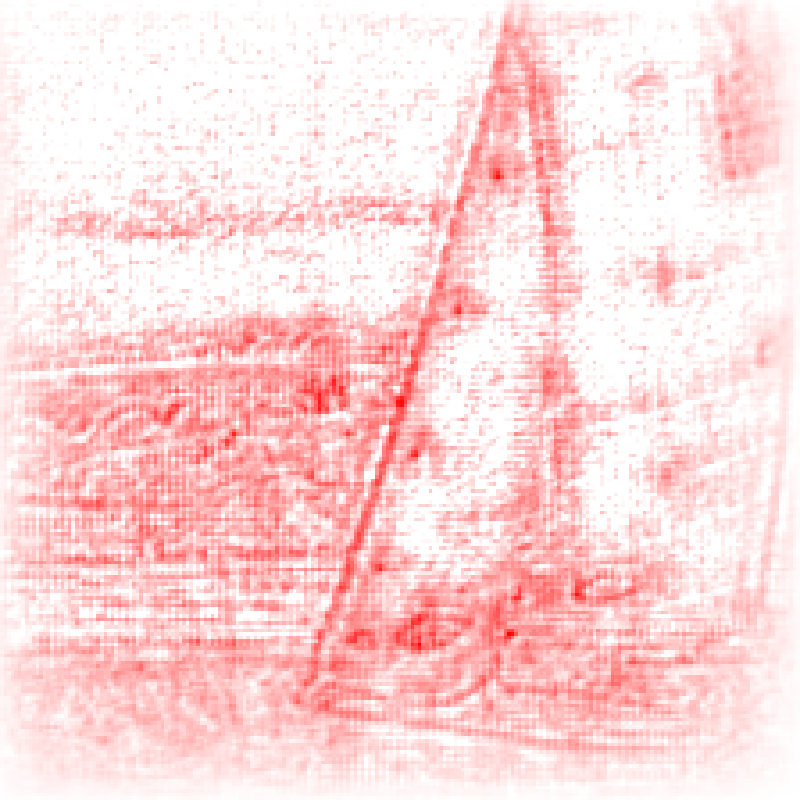
\includegraphics[width=\linewidth]{figures/experiments/saliency_quality/image_0511_ILSVRC2012_val_00035734.JPEG/hybrid_grad_shift_30_max_winnerTakesItAllMaxpool_f0_grad_pp.png}
    \end{minipage}%

    \caption{Saliency map comparison for VGG16 on images from the custom ImageNet-S test subset. Each row shows the predicted class (with confidence), original image, and saliency maps from different methods. Methods include SplitLRP, classical LRP, SplitCAM variants, LayerCAM, and SplitGrad.}
    \label{fig:vgg_saliency_comparison}
\end{figure}


\subsection{Quantitative Analysis on VGG-16}\label{app:vgg_split}

Table~\ref{tab:xai_eval_comprehensive_vgg} contains the complete VGG-16 comparison discussed in Section~\ref{sec:results_vgg}. Selected rows can differ in layer and absolute-value convention; the controlled $\alpha$ sweeps below isolate these choices more directly.

% Source: hiddenMonotonicity (Paper 1), appendix/table_appendix_generated_vgg_full_eval_sorted.tex — numbers verbatim.
\begingroup
\fontsize{8.5}{10}\selectfont
\setlength{\tabcolsep}{3pt}
\renewcommand{\arraystretch}{1.05}
\LongTableContent{
\caption[Comprehensive interpretability evaluation: VGG-16]{Comprehensive interpretability evaluation results (VGG-16; representative configurations, best per method). \emph{wta} denotes winner-takes-it-all max-pooling, and \emph{sc} forward scaling (Section~\ref{sec:stabilization_dc}); layer brackets follow the split-method upper indices of Section~\ref{sec:split_attribution_concept}. For each method configuration the best metric values across the considered layer configurations are highlighted in bold with dark blue shading. PF$^{\mathrm{drop}}$ is score-drop AUC; n/r denotes a result not reported in the paper, and n/a an inapplicable entry.}
    \label{tab:xai_eval_comprehensive_vgg}\label{tab:eval_vgg_main}%
}{%
\begin{longtable}{@{}>{\raggedright\arraybackslash}p{3.6cm}cc cccccc@{}}
    \TableHeading \\
    \toprule
    Method & Layer & Abs & Sel$\downarrow$ & AL$\uparrow$ & PG$\uparrow$ & PF$^{\mathrm{drop}}_5$$\uparrow$ & PF$^{\mathrm{drop}}_{20}$$\uparrow$ & MaxS$\downarrow$ \\
    \midrule
    \endfirsthead

    \multicolumn{9}{c}%
    {{\tablename\ \thetable{} -- continued from previous page}} \\
    \toprule
    Method & Layer & Abs & Sel$\downarrow$ & AL$\uparrow$ & PG$\uparrow$ & PF$^{\mathrm{drop}}_5$$\uparrow$ & PF$^{\mathrm{drop}}_{20}$$\uparrow$ & MaxS$\downarrow$ \\
    \midrule
    \endhead

    \midrule
    \multicolumn{9}{r}{{Continued on next page}} \\
    \midrule
    \endfoot

    \bottomrule
    \endlastfoot

    \multicolumn{9}{c}{\textit{SplitCAM Methods}} \\
    \midrule
    SplitCAM (sc, $\alpha \ 0.4$) & (12, g) & n & 4.720 & \cellbest{\textbf{0.651}} & \cellbest{\textbf{0.912}} & 0.213 & 1.794 & \cellbest{\textbf{0.389}} \\
    SplitCAM (sc, $\alpha \ 0.4$) & (14, g) & n & \cellbest{\textbf{2.727}} & 0.563 & 0.836 & \cellbest{\textbf{0.300}} & \cellbest{\textbf{2.404}} & 1.012 \\
    \cmidrule(lr){1-9}
    SplitCAM (sc, $\alpha \ 0.4$, wta) & (14, g) & n & \cellbest{\textbf{2.761}} & 0.543 & 0.827 & \cellbest{\textbf{0.303}} & \cellbest{\textbf{2.414}} & 1.056 \\
    SplitCAM (sc, $\alpha \ 0.4$, wta) & (26, +, g) & y & 4.711 & \cellbest{\textbf{0.635}} & \cellbest{\textbf{0.938}} & 0.165 & 1.590 & \cellbest{\textbf{0.456}} \\
    \cmidrule(lr){1-9}
    SplitCAM (sc, $\alpha \ 0.5$, wta) & (14, g) & n & \cellbest{\textbf{2.766}} & 0.536 & 0.823 & \cellbest{\textbf{0.303}} & \cellbest{\textbf{2.416}} & 1.056 \\
    SplitCAM (sc, $\alpha \ 0.5$, wta) & (26, +, g) & n & 4.608 & \cellbest{\textbf{0.607}} & \cellbest{\textbf{0.903}} & 0.185 & 1.684 & \cellbest{\textbf{0.566}} \\
    \midrule
    \multicolumn{9}{c}{\textit{SplitGrad Methods}} \\
    \midrule
    SplitGrad ($\alpha \ 0.4$) & (12, +, g) & n & 5.633 & \cellbest{\textbf{0.613}} & \cellbest{\textbf{0.873}} & 0.148 & 1.461 & \cellbest{\textbf{0.364}} \\
    SplitGrad ($\alpha \ 0.4$) & (14, +, g) & y & \cellbest{\textbf{3.429}} & 0.533 & 0.820 & \cellbest{\textbf{0.235}} & \cellbest{\textbf{2.119}} & 0.851 \\
    \cmidrule(lr){1-9}
    SplitGrad ($\alpha \ 0.4$, wta) & (12, +, g) & n & 4.735 & \cellbest{\textbf{0.635}} & \cellbest{\textbf{0.883}} & 0.186 & 1.756 & 0.651 \\
    SplitGrad ($\alpha \ 0.4$, wta) & (14, +, g) & y & \cellbest{\textbf{3.287}} & 0.540 & 0.818 & \cellbest{\textbf{0.249}} & \cellbest{\textbf{2.186}} & 0.857 \\
    \cmidrule(lr){1-9}
    SplitGrad ($\alpha \ 0.5$, wta) & (12, +, g) & y & \cellbest{\textbf{3.379}} & \cellbest{\textbf{0.551}} & 0.859 & \cellbest{\textbf{0.261}} & \cellbest{\textbf{2.220}} & 0.869 \\
    SplitGrad ($\alpha \ 0.5$, wta) & (26, +, g) & y & 4.948 & 0.543 & \cellbest{\textbf{0.899}} & 0.162 & 1.527 & \cellbest{\textbf{0.617}} \\
    \midrule
    \multicolumn{9}{c}{\textit{SplitLRP Methods}} \\
    \midrule
    SplitLRP (sc) & (7, pos) & n & \cellbest{\textbf{3.062}} & 0.092 & \cellbest{\textbf{0.857}} & \cellbest{\textbf{0.296}} & \cellbest{\textbf{2.290}} & 0.865 \\
    SplitLRP (sc) & (19, pos) & n & 4.393 & \cellbest{\textbf{0.600}} & 0.823 & 0.166 & 1.656 & \cellbest{\textbf{0.291}} \\
    \cmidrule(lr){1-9}
    SplitLRP (sc, wta) & (7, pos) & n & \cellbest{\textbf{3.235}} & -0.036 & 0.836 & \cellbest{\textbf{0.296}} & \cellbest{\textbf{2.291}} & 0.866 \\
    SplitLRP (sc, wta) & (26, pos) & y & 5.168 & \cellbest{\textbf{0.588}} & \cellbest{\textbf{0.871}} & 0.151 & 1.473 & \cellbest{\textbf{0.282}} \\
    \midrule
    \multicolumn{9}{c}{\textit{Classical Methods (No Layer Optimization)}} \\
    \midrule
    Deconvolution & 0 & y & 5.435 & 0.468 & 0.629 & 0.204 & 1.715 & 0.956 \\
    DeepLIFT & 0 & y & 4.447 & 0.551 & 0.726 & 0.281 & 1.945 & 1.053 \\
    Feature Ablation & 0 & y & 6.029 & 0.479 & 0.624 & 0.123 & 1.250 & 0.859 \\
    GradientSHAP & 0 & y & 4.808 & 0.552 & 0.783 & 0.261 & 1.862 & 1.142 \\
    IntGrad & 0 & y & 4.838 & 0.554 & 0.797 & 0.262 & 1.851 & 1.069 \\
    Occlusion & 0 & y & 5.214 & 0.499 & 0.716 & 0.130 & 1.217 & 0.699 \\
    GCAM++ & 30 & n & 5.955 & 0.564 & 0.827 & 0.130 & 1.245 & 0.401 \\
    \midrule
    \multicolumn{9}{c}{\textit{Classical Methods (Layer Optimization)}} \\
    \midrule
    Guided Backprop & 2 & n & \cellbest{\textbf{3.276}} & \cellbest{\textbf{0.632}} & 0.883 & \cellbest{\textbf{0.281}} & \cellbest{\textbf{2.302}} & 0.571 \\
    Guided Backprop & 5 & n & 3.448 & 0.614 & \cellbest{\textbf{0.887}} & 0.240 & 2.091 & \cellbest{\textbf{0.375}} \\
    \cmidrule(lr){1-9}
    Guided GCAM & 0 & n & \cellbest{\textbf{4.301}} & \cellbest{\textbf{-0.053}} & \cellbest{\textbf{0.857}} & 0.161 & \cellbest{\textbf{1.459}} & 1.047 \\
    Guided GCAM & 26 & n & 5.130 & -2.635 & 0.843 & \cellbest{\textbf{0.179}} & 1.415 & \cellbest{\textbf{0.947}} \\
    \cmidrule(lr){1-9}
    GCAM & 0 & n & 6.006 & \cellbest{\textbf{0.356}} & \cellbest{\textbf{0.638}} & 0.060 & 0.899 & 1.123 \\
    GCAM & 14 & n & \cellbest{\textbf{5.555}} & 0.306 & 0.580 & \cellbest{\textbf{0.136}} & \cellbest{\textbf{1.525}} & \cellbest{\textbf{0.903}} \\
    \cmidrule(lr){1-9}
    LCAM & 14 & n/a & 2.792 & 0.576 & 0.798 & \cellbest{\textbf{0.317}} & \cellbest{\textbf{2.474}} & \cellbest{\textbf{2.656}} \\
    LCAM & 2 & n/a & \cellbest{\textbf{3.128}} & \cellbest{\textbf{0.580}} & \cellbest{\textbf{0.855}} & 0.300 & 2.191 & 5.508 \\
    \cmidrule(lr){1-9}
    LRP $\gamma=0.25$ & 0 & n & \cellbest{\textbf{3.189}} & \cellbest{\textbf{0.615}} & \cellbest{\textbf{0.680}} & 0.218 & 1.918 & 0.519 \\
    LRP $\gamma=0.25$ & 14 & n & 3.593 & 0.577 & 0.611 & \cellbest{\textbf{0.279}} & \cellbest{\textbf{2.255}} & \cellbest{\textbf{0.491}} \\
    \midrule
    \multicolumn{9}{c}{\textit{Baseline Methods}} \\
    \midrule
    Baseline: Binary Mask & 0 & y & 6.011 & 1.000 & 1.000 & 0.091 & 1.054 & n/r \\
    Baseline: Original Image & 0 & y & 8.770 & -1.699 & 0.572 & 0.061 & 0.619 & n/r \\
    Random Baseline & 0 & y & 3.570 & 0.425 & 0.458 & 0.203 & 1.585 & n/r \\
    \midrule
\end{longtable}%
}
\endgroup


\subsection{Quantitative Analysis on ResNet-18}\label{app:resnet_split}

Table~\ref{tab:xai_eval_comprehensive_res} presents detailed quantitative metrics across all split configurations, baselines, and classical methods for ResNet-18.

% Source: hiddenMonotonicity (Paper 1), appendix/table_appendix_generated_res_full_eval_sorted.tex — numbers verbatim.
% Note: the paper's appendix caption said "ResNet50"; the evaluated model is the ResNet18 of the
% main results (cf. tab:eval_res_main and the paper's main text), so the caption is corrected here.
\begingroup
\fontsize{8.5}{10}\selectfont
\setlength{\tabcolsep}{3pt}
\renewcommand{\arraystretch}{1.05}
\LongTableContent{
\caption[Comprehensive interpretability evaluation: ResNet-18]{Comprehensive interpretability evaluation results (ResNet-18; representative configurations, best per method). Abbreviations as in Table~\ref{tab:eval_res_main}. For each method configuration the best metric values across the considered layer configurations are highlighted in bold with dark blue shading. PF$^{\mathrm{drop}}$ is score-drop AUC; n/r denotes a result not reported in the paper, and n/a an inapplicable entry.}
    \label{tab:xai_eval_comprehensive_res}%
}{%
\begin{longtable}{@{}>{\raggedright\arraybackslash}p{3.6cm}cc cccccc@{}}
    \TableHeading \\
    \toprule
    Method & Layer & Abs & Sel$\downarrow$ & AL$\uparrow$ & PG$\uparrow$ & PF$^{\mathrm{drop}}_5$$\uparrow$ & PF$^{\mathrm{drop}}_{20}$$\uparrow$ & MaxS$\downarrow$ \\
    \midrule
    \endfirsthead

    \multicolumn{9}{c}%
    {{\tablename\ \thetable{} -- continued from previous page}} \\
    \toprule
    Method & Layer & Abs & Sel$\downarrow$ & AL$\uparrow$ & PG$\uparrow$ & PF$^{\mathrm{drop}}_5$$\uparrow$ & PF$^{\mathrm{drop}}_{20}$$\uparrow$ & MaxS$\downarrow$ \\
    \midrule
    \endhead

    \midrule
    \multicolumn{9}{r}{{Continued on next page}} \\
    \midrule
    \endfoot

    \bottomrule
    \endlastfoot

    \multicolumn{9}{c}{\textit{SplitCAM Methods}} \\
    \midrule
    SplitCAM (sc, $\alpha\ 0.3$, wta) & (1.0.2, g) & n & \cellbest{\textbf{3.503}} & 0.487 & 0.747 & \cellbest{\textbf{0.168}} & \cellbest{\textbf{1.395}} & 1.277 \\
    SplitCAM (sc, $\alpha\ 0.3$, wta) & (4.1.2, g) & n & 5.654 & \cellbest{\textbf{0.673}} & \cellbest{\textbf{0.972}} & 0.081 & 0.880 & \cellbest{\textbf{0.233}} \\
    \cmidrule(lr){1-9}
    SplitCAM (sc, $\alpha\ 0.5$, wta) & (2.0.1, g) & n & \cellbest{\textbf{3.682}} & -1.370 & 0.887 & \cellbest{\textbf{0.158}} & \cellbest{\textbf{1.447}} & 1.078 \\
    SplitCAM (sc, $\alpha\ 0.5$, wta) & (4.1.1, +, g) & y & 6.526 & \cellbest{\textbf{0.611}} & \cellbest{\textbf{0.956}} & 0.066 & 0.737 & \cellbest{\textbf{0.187}} \\
    \midrule
    \multicolumn{9}{c}{\textit{SplitGrad Methods}} \\
    \midrule
    SplitGrad ($\alpha\ 0.3$, wta) & (1.0.2, g) & y & \cellbest{\textbf{4.449}} & 0.513 & 0.777 & \cellbest{\textbf{0.149}} & \cellbest{\textbf{1.266}} & 0.813 \\
    SplitGrad ($\alpha\ 0.3$, wta) & (4.1.2, g) & y & 5.663 & \cellbest{\textbf{0.649}} & \cellbest{\textbf{0.972}} & 0.082 & 0.882 & \cellbest{\textbf{0.219}} \\
    \cmidrule(lr){1-9}
    SplitGrad ($\alpha\ 0.5$, wta) & (3.1.1, g) & y & \cellbest{\textbf{3.588}} & 0.559 & 0.880 & \cellbest{\textbf{0.130}} & \cellbest{\textbf{1.366}} & 0.859 \\
    SplitGrad ($\alpha\ 0.5$, wta) & (4.1.2, g) & y & 5.690 & \cellbest{\textbf{0.654}} & \cellbest{\textbf{0.972}} & 0.083 & 0.886 & \cellbest{\textbf{0.230}} \\
    \midrule
    \multicolumn{9}{c}{\textit{SplitLRP Methods}} \\
    \midrule
    SplitLRP (sc, wta) & (conv1, pos) & y & \cellbest{\textbf{6.313}} & \cellbest{\textbf{0.506}} & \cellbest{\textbf{0.587}} & \cellbest{\textbf{0.056}} & \cellbest{\textbf{0.697}} & 0.755 \\
    SplitLRP (sc, wta) & (1.0.2, pos) & y & 6.785 & 0.483 & 0.567 & 0.050 & 0.686 & \cellbest{\textbf{0.696}} \\
    \midrule
    \multicolumn{9}{c}{\textit{Classical Methods (No Layer Optimization)}} \\
    \midrule
    Deconvolution & conv1 & y & 5.474 & 0.478 & 0.666 & 0.151 & 1.177 & 0.618 \\
    GradientSHAP & conv1 & y & 5.269 & 0.527 & 0.779 & 0.166 & 1.227 & 1.074 \\
    GCAM++ & 4.1.2 & n & 6.054 & 0.556 & 0.945 & 0.077 & 0.838 & 0.140 \\
    IntGrad & conv1 & y & 5.265 & 0.528 & 0.777 & 0.167 & 1.226 & 0.994 \\
    Feature Ablation & conv1 & n & 4.655 & 0.136 & 0.684 & 0.188 & 1.388 & 1.077 \\
    Occlusion & conv1 & n & 5.300 & 0.179 & 0.726 & 0.130 & 1.030 & 0.785 \\
    Deconvolution & conv1 & n & 3.934 & 0.484 & 0.666 & 0.147 & 1.203 & 0.751 \\
    \midrule
    \multicolumn{9}{c}{\textit{Classical Methods (Layer Optimization)}} \\
    \midrule
    GCAM & 2.0.1 & y & \cellbest{\textbf{4.003}} & 0.450 & 0.678 & 0.052 & \cellbest{\textbf{1.024}} & 0.738 \\
    GCAM & 4.1.2 & n & 6.070 & \cellbest{\textbf{0.554}} & \cellbest{\textbf{0.945}} & \cellbest{\textbf{0.076}} & 0.829 & \cellbest{\textbf{0.131}} \\
    \cmidrule(lr){1-9}
    Guided GCAM & 4.0.2 & n & 4.929 & \cellbest{\textbf{0.742}} & 0.866 & 0.119 & 1.008 & 0.687 \\
    Guided GCAM & 4.1.2 & n & \cellbest{\textbf{3.843}} & 0.717 & \cellbest{\textbf{0.883}} & \cellbest{\textbf{0.129}} & \cellbest{\textbf{1.096}} & \cellbest{\textbf{0.612}} \\
    \cmidrule(lr){1-9}
    LCAM & 2.0.2 & n & \cellbest{\textbf{3.690}} & 0.549 & 0.865 & \cellbest{\textbf{0.144}} & \cellbest{\textbf{1.428}} & 0.913 \\
    LCAM & 4.1.1 & n & 5.661 & \cellbest{\textbf{0.664}} & \cellbest{\textbf{0.971}} & 0.083 & 0.890 & \cellbest{\textbf{0.227}} \\
    \cmidrule(lr){1-9}
    LRP $\gamma=0.25$ & conv1 & y & \cellbest{\textbf{3.550}} & \cellbest{\textbf{0.656}} & 0.852 & \cellbest{\textbf{0.213}} & \cellbest{\textbf{1.737}} & 0.521 \\
    LRP $\gamma=0.25$ & 4.1.1 & n & 5.649 & 0.630 & \cellbest{\textbf{0.965}} & 0.081 & 0.877 & \cellbest{\textbf{0.200}} \\
    \cmidrule(lr){1-9}
    Guided Backprop & conv1 & n & \cellbest{\textbf{3.517}} & \cellbest{\textbf{0.621}} & 0.867 & \cellbest{\textbf{0.212}} & \cellbest{\textbf{1.757}} & 0.459 \\
    Guided Backprop & 3.1.2 & n & 3.874 & 0.582 & \cellbest{\textbf{0.938}} & 0.121 & 1.307 & \cellbest{\textbf{0.213}} \\
    \midrule
    \multicolumn{9}{c}{\textit{Baseline Methods}} \\
    \midrule
    Baseline: Original Image & conv1 & y & 8.351 & -1.699 & 0.572 & 0.049 & 0.435 & n/r \\
    Baseline: Binary Mask & conv1 & y & 5.964 & 1.000 & 1.000 & 0.067 & 0.739 & n/r \\
    Random Baseline & n/a & y & 4.071 & 0.425 & 0.440 & 0.147 & 1.067 & n/r \\
    \midrule
    \end{longtable}%
}
\endgroup


\section{Stabilization Ablations for the Split Methods}\label{app:ablation}

These ablation studies examine the effect of the proposed stabilization techniques for the forward and backward pass, as well as the influence of the selected max-pooling implementation (Section~\ref{sec:stabilization_dc}).

\subsection{Backward-Pass Stabilization}\label{app:backward_ablation}

Table~\ref{tab:alpha_comparison_by_method} gives the full $\alpha$ grid underlying Section~\ref{subsec:alpha_ablation}. Layer-14 configurations show smaller or adverse changes in some metrics. Convex and winner-takes-it-all max-pooling differ little near $\alpha=0.5$ and more at lower values; their ranking depends on configuration and metric.

\paragraph{Unresolved source-table discrepancy.}
For SplitCAM with scaling, $\alpha=0.4$, winner-takes-it-all pooling and absolute-value configuration $(26,+,g)$, Table~\ref{tab:xai_eval_comprehensive_vgg} reports PF$^{\mathrm{drop}}_{20}=1.590$ and MaxS$=0.456$, versus $1.5849$ and $0.4573$ in Table~\ref{tab:alpha_comparison_by_method}. These source-table values remain unchanged: the per-image results needed to resolve their discrepancy are unavailable, leaving its cause unknown.

% Source: hiddenMonotonicity (Paper 1), appendix/table_ppendix_alpha_combined.tex — numbers verbatim, restyled to booktabs.
\begin{table}[htb!]
    \centering
    \footnotesize
    \setlength{\tabcolsep}{5pt}
    \renewcommand{\arraystretch}{1.2}
    \caption{Alpha ablation as performed in Section~\ref{sec:ablations} across four SplitGrad and SplitCAM configurations of layers $14$ and $26$, respectively. The notation is similar to Table~\ref{tab:eval_vgg_main}.}
    \label{tab:alpha_comparison_by_method}
    \begin{adjustbox}{max width=\linewidth}
\begin{tabular}{ll cccccc}
    \toprule
    \textbf{Method} & \textbf{Metric} & $\alpha \ 0.50$ & $\alpha \ 0.45$ & $\alpha \ 0.40$ & $\alpha \ 0.35$ & $\alpha \ 0.30$ & $\alpha \ 0.00$ \\
    \midrule
    \multirow{4}{*}{\begin{tabular}[c]{@{}l@{}}\textbf{SplitGrad (wta)}\\(26, g), abs\end{tabular}} & PG$\uparrow$ & 0.8975 & 0.9064 & 0.9470 & \cellbest{\textbf{0.9558}} & 0.8887 & 0.4011 \\
     & AL$\uparrow$ & 0.5434 & 0.5476 & 0.6051 & \cellbest{\textbf{0.6169}} & 0.5346 & 0.4486 \\
     & MaxS$\downarrow$ & 0.6160 & 0.6071 & 0.4399 & 0.2382 & 0.3344 & \cellbest{\textbf{0.0283}} \\
     & PF$^{\mathrm{drop}}_{20}$ $\uparrow$ & 1.5270 & 1.5337 & \cellbest{\textbf{1.5808}} & 1.4476 & 1.3171 & 1.2471 \\
    \midrule
    \multirow{4}{*}{\begin{tabular}[c]{@{}l@{}}\textbf{SplitGrad}\\(26, g), abs\end{tabular}} & PG$\uparrow$ & 0.8975 & 0.9064 & \cellbest{\textbf{0.9470}} & 0.9099 & 0.2827 & 0.6413 \\
     & AL$\uparrow$ & 0.5434 & 0.5476 & \cellbest{\textbf{0.6037}} & 0.5216 & 0.4245 & 0.4563 \\
     & MaxS$\downarrow$ & 0.6171 & 0.6102 & 0.4426 & 0.3864 & 0.0622 & \cellbest{\textbf{0.0079}} \\
     & PF$^{\mathrm{drop}}_{20}$ $\uparrow$ & 1.5272 & 1.5333 & \cellbest{\textbf{1.5876}} & 1.3702 & 0.2431 & 0.5755 \\
    \midrule
    \multirow{4}{*}{\begin{tabular}[c]{@{}l@{}}\textbf{SplitGrad (wta)}\\(14, g), abs\end{tabular}} & PG$\uparrow$ & 0.8198 & 0.8198 & 0.8198 & \cellbest{\textbf{0.8322}} & 0.8127 & 0.7898 \\
     & AL$\uparrow$ & \cellbest{\textbf{0.5403}} & 0.5403 & 0.5402 & 0.5006 & 0.4936 & 0.4857 \\
     & MaxS$\downarrow$ & 0.8579 & 0.8597 & 0.8584 & 0.0875 & 0.0677 & \cellbest{\textbf{0.0481}} \\
     & PF$^{\mathrm{drop}}_{20}$ $\uparrow$ & 2.1887 & \cellbest{\textbf{2.1894}} & 2.1869 & 1.8740 & 1.8304 & 1.7684 \\
    \midrule
    \multirow{4}{*}{\begin{tabular}[c]{@{}l@{}}\textbf{SplitGrad}\\(14, g), abs\end{tabular}} & PG$\uparrow$ & 0.8198 & \cellbest{\textbf{0.8198}} & 0.8180 & 0.7951 & 0.8004 & 0.7968 \\
     & AL$\uparrow$ & 0.5403 & \cellbest{\textbf{0.5403}} & 0.5330 & 0.5054 & 0.4926 & 0.4847 \\
     & MaxS$\downarrow$ & 0.8618 & 0.8584 & 0.8478 & 0.1103 & 0.0662 & \cellbest{\textbf{0.0301}} \\
     & PF$^{\mathrm{drop}}_{20}$ $\uparrow$ & \cellbest{\textbf{2.1894}} & 2.1891 & 2.1185 & 1.3425 & 1.2959 & 1.1927 \\
    \midrule
    \multirow{4}{*}{\begin{tabular}[c]{@{}l@{}}\textbf{SplitCAM (sc, wta)}\\(26, +, g), abs\end{tabular}} & PG$\uparrow$ & 0.8675 & 0.8675 & \cellbest{\textbf{0.9382}} & 0.9329 & 0.6131 & 0.8551 \\
     & AL$\uparrow$ & 0.5501 & 0.5535 & 0.6347 & \cellbest{\textbf{0.6627}} & 0.4033 & 0.5133 \\
     & MaxS$\downarrow$ & 0.6906 & 0.6820 & 0.4573 & 0.2645 & 0.2511 & \cellbest{\textbf{0.1196}} \\
     & PF$^{\mathrm{drop}}_{20}$ $\uparrow$ & 1.6067 & \cellbest{\textbf{1.6085}} & 1.5849 & 1.4989 & 0.8534 & 1.5071 \\
    \midrule
    \multirow{4}{*}{\begin{tabular}[c]{@{}l@{}}\textbf{SplitCAM (sc)}\\(26, +, g), abs\end{tabular}} & PG$\uparrow$ & 0.8940 & 0.8905 & \cellbest{\textbf{0.9346}} & 0.6466 & 0.8251 & 0.8604 \\
     & AL$\uparrow$ & 0.5595 & 0.5636 & \cellbest{\textbf{0.6363}} & 0.4015 & 0.4977 & 0.5114 \\
     & MaxS$\downarrow$ & 0.6738 & 0.6640 & 0.4520 & 0.3729 & 0.1102 & \cellbest{\textbf{0.1062}} \\
     & PF$^{\mathrm{drop}}_{20}$ $\uparrow$ & 1.5902 & \cellbest{\textbf{1.5978}} & 1.5906 & 0.9076 & 1.2784 & 1.3605 \\
    \midrule
    \multirow{4}{*}{\begin{tabular}[c]{@{}l@{}}\textbf{SplitCAM (sc, wta)}\\(14, g)\end{tabular}} & PG$\uparrow$ & 0.8251 & 0.8251 & \cellbest{\textbf{0.8269}} & 0.7880 & 0.7809 & 0.7703 \\
     & AL$\uparrow$ & 0.5363 & 0.5363 & \cellbest{\textbf{0.5435}} & 0.5338 & 0.5286 & 0.5225 \\
     & MaxS$\downarrow$ & 1.0566 & 1.0569 & 1.0489 & \cellbest{\textbf{0.1620}} & 0.1625 & 0.1630 \\
     & PF$^{\mathrm{drop}}_{20}$ $\uparrow$ & 2.4128 & 2.4130 & \cellbest{\textbf{2.4135}} & 1.9014 & 1.8613 & 1.8731 \\
    \midrule
    \multirow{4}{*}{\begin{tabular}[c]{@{}l@{}}\textbf{SplitCAM (sc)}\\(14, g)\end{tabular}} & PG$\uparrow$ & 0.8251 & 0.8251 & \cellbest{\textbf{0.8428}} & 0.7756 & 0.7686 & 0.7756 \\
     & AL$\uparrow$ & 0.5363 & 0.5363 & \cellbest{\textbf{0.5626}} & 0.5363 & 0.5271 & 0.5208 \\
     & MaxS$\downarrow$ & 1.0552 & 1.0593 & 1.0136 & 0.1629 & 0.1585 & \cellbest{\textbf{0.1555}} \\
     & PF$^{\mathrm{drop}}_{20}$ $\uparrow$ & 2.4171 & \cellbest{\textbf{2.4172}} & 2.4065 & 1.5032 & 1.5082 & 1.5139 \\
    \bottomrule
    \end{tabular}
\end{adjustbox}
\end{table}


\subsection{Forward-stabilization grids}

Tables~\ref{tab:alpha_comparison_none} and~\ref{tab:alpha_comparison_shift} give the full unstabilized and shift-stabilized SplitCAM grids discussed in Section~\ref{app:forward_ablation}.

% Source: hiddenMonotonicity (Paper 1), appendix/table_alpha_none.tex — numbers verbatim, restyled to booktabs.
% The paper's green cell highlighting is rendered here as a star marker (*) since the thesis
% preamble does not load colortbl.
\begin{table}[htbp]
    \centering
    \footnotesize
    \setlength{\tabcolsep}{5pt}
    \renewcommand{\arraystretch}{1.2}
    \caption{Alpha ablation for scale normalization across four SplitCAM configurations of layers 14 and 26. Here, in the forward pass \emph{no} stabilization is applied. Notation and structure are similar to Table~\ref{tab:alpha_comparison_by_method}. Light blue entries marked with $^{\ast}$ indicate better performance of the method compared to the default variant with scale stabilization in the forward pass.}
    \label{tab:alpha_comparison_none}
    \begin{adjustbox}{max width=\linewidth}
\begin{tabular}{ll cccccc}
    \toprule
    \textbf{Method} & \textbf{Metric} & $\alpha \ 0.50$ & $\alpha \ 0.45$ & $\alpha \ 0.40$ & $\alpha \ 0.35$ & $\alpha \ 0.30$ & $\alpha \ 0.00$ \\
    \midrule
    \multirow{4}{*}{\begin{tabular}[c]{@{}l@{}}\textbf{SplitCAM (sc, wta)}\\(26, +, g), abs\end{tabular}} & PG$\uparrow$ & 0.7686 & 0.7686 & 0.8632 & \cellbest{\textbf{0.8712}} & 0.3441 & 0.5453 \\
     & AL$\uparrow$ & 0.5374 & 0.5412 & 0.5943 & \cellbest{\textbf{0.6118}} & 0.3595 & 0.4569 \\
     & MaxS$\downarrow$ & \cellapprox{0.6578}$^{\ast}$ & \cellapprox{0.6507}$^{\ast}$ & 0.4841 & 0.2873 & \cellapprox{0.1918}$^{\ast}$ & \cellapprox{\cellbest{\textbf{0.0135}}}$^{\ast}$ \\
     & PF$^{\mathrm{drop}}_{20}$ $\uparrow$ & 1.2744 & 1.2859 & \cellbest{\textbf{1.3209}} & 1.1792 & 0.4430 & 0.6527 \\
    \midrule
    \multirow{4}{*}{\begin{tabular}[c]{@{}l@{}}\textbf{SplitCAM (sc)}\\(26, +, g), abs\end{tabular}} & PG$\uparrow$ & 0.7565 & 0.7565 & \cellbest{\textbf{0.8451}} & 0.3783 & 0.4507 & 0.4970 \\
     & AL$\uparrow$ & 0.5346 & 0.5384 & \cellbest{\textbf{0.5897}} & 0.3663 & 0.4420 & 0.4545 \\
     & MaxS$\downarrow$ & \cellapprox{0.6604}$^{\ast}$ & \cellapprox{0.6512}$^{\ast}$ & 0.4985 & \cellapprox{0.3077}$^{\ast}$ & \cellapprox{0.0279}$^{\ast}$ & \cellapprox{\cellbest{\textbf{0.0043}}}$^{\ast}$ \\
     & PF$^{\mathrm{drop}}_{20}$ $\uparrow$ & 1.2680 & 1.2856 & \cellbest{\textbf{1.3295}} & 0.5912 & 0.4906 & 0.5563 \\
    \midrule
    \multirow{4}{*}{\begin{tabular}[c]{@{}l@{}}\textbf{SplitCAM (sc, wta)}\\(14, g)\end{tabular}} & PG$\uparrow$ & \cellapprox{\cellbest{\textbf{0.8491}}}$^{\ast}$ & \cellapprox{0.8491}$^{\ast}$ & \cellapprox{0.8491}$^{\ast}$ & 0.7867 & \cellapprox{0.7847}$^{\ast}$ & 0.7686 \\
     & AL$\uparrow$ & 0.5324 & 0.5321 & \cellbest{\textbf{0.5406}} & 0.5306 & 0.5261 & 0.5200 \\
     & MaxS$\downarrow$ & 1.0834 & 1.0814 & 1.0885 & \cellbest{\textbf{0.2271}} & 0.2309 & 0.2384 \\
     & PF$^{\mathrm{drop}}_{20}$ $\uparrow$ & \cellapprox{2.4454}$^{\ast}$ & \cellapprox{2.4482}$^{\ast}$ & \cellapprox{\cellbest{\textbf{2.4486}}}$^{\ast}$ & \cellapprox{1.9588}$^{\ast}$ & \cellapprox{1.9193}$^{\ast}$ & \cellapprox{1.9349}$^{\ast}$ \\
    \midrule
    \multirow{4}{*}{\begin{tabular}[c]{@{}l@{}}\textbf{SplitCAM (sc)}\\(14, g)\end{tabular}} & PG$\uparrow$ & 0.7746 & 0.7767 & \cellbest{\textbf{0.7847}} & 0.5855 & 0.5594 & 0.5573 \\
     & AL$\uparrow$ & 0.4003 & 0.4144 & \cellbest{\textbf{0.5517}} & 0.5300 & 0.5209 & 0.5137 \\
     & MaxS$\downarrow$ & 1.5733 & 1.5627 & 1.5443 & \cellbest{\textbf{1.2661}} & 1.3939 & 1.4272 \\
     & PF$^{\mathrm{drop}}_{20}$ $\uparrow$ & 2.1298 & \cellbest{\textbf{2.1384}} & 2.1371 & \cellapprox{1.6669}$^{\ast}$ & \cellapprox{1.6793}$^{\ast}$ & \cellapprox{1.6740}$^{\ast}$ \\
    \bottomrule
    \end{tabular}
\end{adjustbox}
\end{table}

% Source: hiddenMonotonicity (Paper 1), appendix/table_alpha_shift.tex — numbers verbatim, restyled to booktabs.
% The paper's green cell highlighting is rendered here as a star marker (*) since the thesis
% preamble does not load colortbl.
\begin{table}[htbp]
    \centering
    \footnotesize
    \setlength{\tabcolsep}{5pt}
    \renewcommand{\arraystretch}{1.2}
    \caption[Alpha ablation with shift normalization]{Alpha ablation for scaling normalization across four SplitCAM configurations of layers 14 and 26. Here, in the forward pass shift normalization is applied. Notation and structure are similar to Table~\ref{tab:alpha_comparison_by_method}. Light blue entries marked with $^{\ast}$ indicate better performance of the method compared to the default variant with scale stabilization in the forward pass.}
    \label{tab:alpha_comparison_shift}
\TableContent{
    \begin{adjustbox}{max width=\linewidth}
\begin{tabular}{ll cccccc}
    \toprule
    \textbf{Method} & \textbf{Metric} & $\alpha \ 0.50$ & $\alpha \ 0.45$ & $\alpha \ 0.40$ & $\alpha \ 0.35$ & $\alpha \ 0.30$ & $\alpha \ 0.00$ \\
    \midrule
    \multirow{4}{*}{\begin{tabular}[c]{@{}l@{}}\textbf{SplitCAM (sc, wta)}\\(26, +, g), abs\end{tabular}} & PG$\uparrow$ & 0.8330 & 0.8149 & 0.7968 & \cellbest{\textbf{0.9235}} & 0.6036 & \cellapprox{0.8592}$^{\ast}$ \\
     & AL$\uparrow$ & 0.5242 & 0.5203 & 0.5147 & \cellbest{\textbf{0.6549}} & 0.3968 & 0.5093 \\
     & MaxS$\downarrow$ & \cellapprox{0.6180}$^{\ast}$ & \cellapprox{0.6182}$^{\ast}$ & 0.6509 & 0.3104 & 0.2791 & \cellbest{\textbf{0.1665}} \\
     & PF$^{\mathrm{drop}}_{20}$ $\uparrow$ & \cellapprox{\cellbest{\textbf{1.6804}}}$^{\ast}$ & \cellapprox{1.6646}$^{\ast}$ & 1.5065 & 1.4962 & \cellapprox{0.8896}$^{\ast}$ & \cellapprox{1.5405}$^{\ast}$ \\
    \midrule
    \multirow{4}{*}{\begin{tabular}[c]{@{}l@{}}\textbf{SplitCAM (sc)}\\(26, +, g), abs\end{tabular}} & PG$\uparrow$ & 0.8330 & 0.8149 & 0.7988 & 0.5654 & \cellapprox{0.8431}$^{\ast}$ & \cellapprox{\cellbest{\textbf{0.8652}}}$^{\ast}$ \\
     & AL$\uparrow$ & \cellbest{\textbf{0.5242}} & 0.5203 & 0.5076 & 0.3736 & 0.4949 & 0.5094 \\
     & MaxS$\downarrow$ & \cellapprox{0.6129}$^{\ast}$ & \cellapprox{0.6168}$^{\ast}$ & 0.6494 & 0.3820 & 0.1686 & \cellbest{\textbf{0.1664}} \\
     & PF$^{\mathrm{drop}}_{20}$ $\uparrow$ & \cellapprox{\cellbest{\textbf{1.6804}}}$^{\ast}$ & \cellapprox{1.6646}$^{\ast}$ & 1.5105 & 0.8714 & \cellapprox{1.4289}$^{\ast}$ & \cellapprox{1.4765}$^{\ast}$ \\
    \midrule
    \multirow{4}{*}{\begin{tabular}[c]{@{}l@{}}\textbf{SplitCAM (sc, wta)}\\(14, g)\end{tabular}} & PG$\uparrow$ & \cellapprox{\cellbest{\textbf{0.8310}}}$^{\ast}$ & \cellapprox{0.8310}$^{\ast}$ & \cellapprox{0.8310}$^{\ast}$ & \cellapprox{0.7887}$^{\ast}$ & \cellapprox{0.7827}$^{\ast}$ & \cellapprox{0.7726}$^{\ast}$ \\
     & AL$\uparrow$ & 0.5312 & 0.5312 & \cellbest{\textbf{0.5376}} & 0.5315 & 0.5264 & 0.5203 \\
     & MaxS$\downarrow$ & \cellapprox{1.0562}$^{\ast}$ & \cellapprox{1.0521}$^{\ast}$ & 1.0649 & \cellbest{\textbf{0.1633}} & 0.1641 & 0.1642 \\
     & PF$^{\mathrm{drop}}_{20}$ $\uparrow$ & \cellapprox{\cellbest{\textbf{2.4412}}}$^{\ast}$ & \cellapprox{2.4412}$^{\ast}$ & \cellapprox{2.4400}$^{\ast}$ & \cellapprox{1.9306}$^{\ast}$ & \cellapprox{1.8953}$^{\ast}$ & \cellapprox{1.9059}$^{\ast}$ \\
    \midrule
    \multirow{4}{*}{\begin{tabular}[c]{@{}l@{}}\textbf{SplitCAM (sc)}\\(14, g)\end{tabular}} & PG$\uparrow$ & \cellapprox{0.8310}$^{\ast}$ & \cellapprox{0.8310}$^{\ast}$ & \cellapprox{\cellbest{\textbf{0.8431}}}$^{\ast}$ & 0.7746 & \cellapprox{0.7706}$^{\ast}$ & \cellapprox{0.7807}$^{\ast}$ \\
     & AL$\uparrow$ & 0.5311 & 0.5312 & \cellbest{\textbf{0.5580}} & 0.5337 & 0.5245 & 0.5183 \\
     & MaxS$\downarrow$ & 1.0554 & \cellapprox{1.0568}$^{\ast}$ & 1.0198 & 0.1641 & 0.1587 & \cellbest{\textbf{0.1570}} \\
     & PF$^{\mathrm{drop}}_{20}$ $\uparrow$ & \cellapprox{\cellbest{\textbf{2.4412}}}$^{\ast}$ & \cellapprox{2.4411}$^{\ast}$ & \cellapprox{2.4318}$^{\ast}$ & \cellapprox{1.5187}$^{\ast}$ & \cellapprox{1.5222}$^{\ast}$ & \cellapprox{1.5329}$^{\ast}$ \\
    \bottomrule
    \end{tabular}
\end{adjustbox}
}%
\end{table}


\section{Additional Results}\label{ptnb:app:results}

The validation, test and VOC tables are generated by one pipeline from the declared grids and the selection rules of Section~\ref{ptnb:app:protocol}.

\paragraph{Configuration symbols.}\label{ptnb:app:config-symbols}
Parameter grids and baseline recipes appear in Table~\ref{ptnb:tab:main-search-grid}. The configuration columns use the following parameters. \ac{rg}, \ac{rg}+Eq and \ac{sg}: temperature $\tau$, activation-side risk aversion $\lambda$, attention-logit risk aversion $\lambda_{\mathrm{sm}}$, \ac{ptnbADF} input variance $\sigma^2$, \ac{lrp} stabilizer $\varepsilon$, stream weights $(\alpha,\beta)$, noisy-observation gate $\tilde\Phi$, and the number $N$ of transformed inputs averaged by \ac{rg}+Eq. SmoothGrad: $N$ noisy samples with noise standard deviation $\sigma$ relative to the input range ($\sigma/\mathrm{range}$). Integrated Gradients: $N_{\mathrm{steps}}$ integration steps. DAVE: $N$ transformed inputs with rotations up to $\theta_{\max}$ degrees, shifts up to $s_{\max}$ of the image extent, and variance-preserving Gaussian noise of interpolation weight up to $t_{\max}$. AttnLRP: $\gamma$-rule parameters $\gamma_{\mathrm{conv}}$ and $\gamma_{\mathrm{lin}}$ of the convolutional and linear layers and the stabilizer $\varepsilon_{\mathrm{attn}}$ of the attention layers. LIME and KernelSHAP: $N$ perturbation samples. Row labels in parentheses give the selection criterion (\texttt{loc}, \texttt{faith}); single-configuration methods have no criterion.

\subsection{Validation selections}\label{ptnb:app:val-selection}

Table~\ref{ptnb:tab:val-selection-all} gives both rank-sums for each validation choice on the 50-image split. The full test tables identify the selected configurations.

\begin{table}[htbp]
    \centering
    \caption[Validation selection on ViT-B/16, VGG-16 and ResNet-50]{ViT-B/16, VGG-16 and ResNet-50: validation rank-sums within each method, lower is better. Each pair reports localization and faithfulness rank-sums for the row selected by the named criterion (Section~\ref{ptnb:app:selection}); anchors are fixed reference configurations.}
    \label{ptnb:tab:val-selection-all}
\TableContent{
    \small
    \setlength{\tabcolsep}{3pt}
    \begin{tabular}{@{}ll rc rc rc@{}}
\toprule
Method & Selection & \multicolumn{2}{c}{ViT-B/16} & \multicolumn{2}{c}{VGG-16} & \multicolumn{2}{c}{ResNet-50} \\
 & & $n$ & $(r_{\mathrm{loc}},r_{\mathrm{faith}})$ & $n$ & $(r_{\mathrm{loc}},r_{\mathrm{faith}})$ & $n$ & $(r_{\mathrm{loc}},r_{\mathrm{faith}})$ \\
\midrule
SmGrad & loc & 3 & $(3.5,3)$ & 3 & $(3,3)$ & 3 & $(4,5)$ \\
 & faith &  & $(3.5,3)$ &  & $(3,3)$ &  & $(8,4)$ \\
\addlinespace
IntGrad & loc & 4 & $(3.5,4)$ & 4 & $(6,3)$ & 4 & $(3,6)$ \\
 & faith &  & $(3.5,4)$ &  & $(6,3)$ &  & $(7.5,6)$ \\
\addlinespace
LRP-$\varepsilon$ & loc & 7 & $(5.5,7)$ & 7 & $(6,9)$ & 7 & $(5.5,9)$ \\
 & faith &  & $(6.5,3)$ &  & $(6,4)$ &  & $(8,4)$ \\
\addlinespace
LRP-$\gamma$ & loc & 15 & $(6,25)$ & 30 & $(13,43)$ & 30 & $(12.5,33)$ \\
 & faith &  & $(32,12)$ &  & $(36,5)$ &  & $(36,22.5)$ \\
\addlinespace
AttnLRP & loc & 11 & $(3,29)$ & --- & --- & --- & --- \\
 & faith &  & $(14,7)$ &  & --- &  & --- \\
\addlinespace
DAVE & loc/faith & 54 & $(14,6)$ & --- & --- & --- & --- \\
\addlinespace
AR & loc/faith & 4 & $(3.5,3)$ & --- & --- & --- & --- \\
\addlinespace
SG & loc & --- & --- & 40 & $(37,10)$ & --- & --- \\
 & faith &  & --- &  & $(49.5,6)$ &  & --- \\
\addlinespace
RG & loc & 672 & $(47,788)$ & 544 & $(78,194)$ & 544 & $(19,224)$ \\
 & faith &  & $(1156,22)$ &  & $(173.5,5)$ &  & $(466,38)$ \\
 & anchor &  & $(1420,344)$ &  & $(339,60)$ &  & $(212.5,140)$ \\
\addlinespace
RG+Eq & loc & 16 & $(6.5,29)$ & --- & --- & --- & --- \\
 & faith &  & $(14,11)$ &  & --- &  & --- \\
 & anchor &  & $(47,31)$ &  & --- &  & --- \\
\bottomrule
\end{tabular}
\par\smallskip\noindent
$n$: declared grid size (Table~\ref{ptnb:tab:main-search-grid}); ranks use admitted configurations (Section~\ref{ptnb:app:selection}).
Configurations are identified by method and selection in Tables~\ref{ptnb:tab:test-ci-vit}, \ref{ptnb:tab:test-ci-vgg} and~\ref{ptnb:tab:test-ci-resnet}.
Fixed methods have one configuration and n/a rank-sums. A dash marks an architecture on which the method was not evaluated.

}%
\end{table}
\AliasLabel{ptnb:tab:val-selection-vit}{ptnb:tab:val-selection-all}
\AliasLabel{ptnb:tab:val-selection-vgg}{ptnb:tab:val-selection-all}
\AliasLabel{ptnb:tab:val-selection-resnet}{ptnb:tab:val-selection-all}

\subsection{Test results with confidence intervals}\label{ptnb:app:test-ci}

Table~\ref{ptnb:tab:test-ci-vit} and Tables~\ref{ptnb:tab:test-ci-vgg}--\ref{ptnb:tab:test-ci-resnet} report all 565-image test rows: \texttt{loc}/\texttt{faith} selections, anchors and fixed configurations. Confidence intervals and highlighting follow Table~\ref{ptnb:tab:test-ci-vit}; ViT-B/16 runtimes appear in Section~\ref{sec:results_vit}.

\appneedspace{8\baselineskip}
\begin{center}
    \captionsetup{hypcap=false}
    \captionof{table}[VGG-16: full ImageNet-S results with confidence intervals]{VGG-16, ImageNet-S test split: all rows with 95\% bootstrap confidence intervals,
    as in Table~\ref{ptnb:tab:test-ci-vit}.}
    \label{ptnb:tab:test-ci-vgg}
\end{center}
\captionsetup{hypcap=true}
\appinputgenci{tables/ptnb_v2/generated/test_vgg16_ci_longtable}

\appneedspace{8\baselineskip}
\begin{center}
    \captionsetup{hypcap=false}
    \captionof{table}[ResNet-50: full ImageNet-S results with confidence intervals]{ResNet-50, ImageNet-S test split: all rows with 95\% bootstrap confidence
    intervals, as in Table~\ref{ptnb:tab:test-ci-vit}.}
    \label{ptnb:tab:test-ci-resnet}
\end{center}
\captionsetup{hypcap=true}
\appinputgenci{tables/ptnb_v2/generated/test_resnet50_ci_longtable}

\subsection{Cross-Dataset Evaluation: Pascal VOC 2012}\label{ptnb:app:voc-cross-data}\label{app:voc-cross-data}
Table~\ref{ptnb:tab:eval-vit-voc} gives all rows underlying the transfer comparison in Section~\ref{ptnb:sec:experiments}.

\paragraph{Dataset.}
We use Pascal VOC 2012~\parencite{Everingham2010voc} segmentation annotations\footnote{Release statistics: \url{https://www.robots.ox.ac.uk/~vgg/projects/pascal/VOC/voc2012/dbstats.html}.}: the trainval pool of
$2{,}913$ images with pixel-accurate \texttt{Seg\-mentationClass} masks across $20$ foreground
classes plus background. Each image is expanded to one (image, foreground-class) sample per
distinct VOC class label present in its mask, yielding $3{,}422$ total samples after dropping the
\texttt{person} class (no faithful ImageNet-1K target exists for it) and discarding sliver masks
whose pixel area on the \emph{original} (pre-resize) annotation is below $64$ pixels. Each (image,
class) sample carries the same input image and an explanation target equal to the most semantically
central ImageNet-1K index for that VOC class (e.g.\ \texttt{horse}$\,\to\,$\textsc{n02389026
sorrel}; \texttt{tvmonitor}$\,\to\,$\textsc{n03782006 monitor}); the curated mapping is part of the
released code.

\paragraph{Per-image disjoint val/test split.} The trainval pool is partitioned randomly with seed $42$ at the \emph{image} level (not the (image,
class) level) into a $1{:}5$ val/test split: the trainval stems are shuffled deterministically and
the first $1/6$ is assigned to val. All (image, class) samples for a given image stay in the same
partition, preventing the same image from appearing in both tuning and test sets. As on
ImageNet-S, samples whose object mask lies entirely outside the $224{\times}224$ center crop are
excluded after the split (18 val and 105 test samples). The validation split contains $460$ images and $556$ image--class samples; the test split contains $2{,}293$ images and $2{,}743$ samples.

\paragraph{Pixel masks for localization.} \ac{ptnbAttrLoc}, \ac{ptnbPG}, and Top-$k$ Intersection use each image--class sample's binary VOC2012 segmentation mask, rewarding only foreground pixels rather than background within a bounding box. NEAREST resizing and $224{\times}224$ center-cropping match the input pipeline (\texttt{Resize(256)$\,\to\,$CenterCrop(224)}); Quantus~\parencite{Hedstrom2023} receives this mask unchanged alongside the attribution map.

\paragraph{Tuning protocol.}
Every ViT-B/16 baseline configuration in Table~\ref{ptnb:tab:main-search-grid} is evaluated on the $556$-sample VOC validation pool; the \texttt{loc} and \texttt{faith} criteria of Section~\ref{ptnb:app:selection} select rows for the $2{,}743$-sample test pool. \ac{rg} and \ac{rg}+Eq transfer their ImageNet-S anchors and both selected configurations unchanged. To save compute, VOC evaluates only localization and faithfulness, omitting MaxS, AvgS and runtime. Per-metric tests (Section~\ref{ptnb:app:stats}) count significant wins, losses and undetected differences; the last category does not establish equivalence.

\appneedspace{8\baselineskip}
\begin{center}
    \captionsetup{hypcap=false}
    \captionof{table}[ViT-B/16 on the Pascal VOC 2012 test pool]{ViT-B/16 on Pascal VOC 2012: all $2{,}743$ test image--class records from $2{,}293$ images, with record-weighted means and 95\% image-cluster bootstrap confidence intervals. The transfer and baseline-selection protocol is specified above; only localization and faithfulness were evaluated. Metrics: Table~\ref{ptnb:tab:eval-vit}; configuration symbols and row labels: Section~\ref{ptnb:app:config-symbols}.}
    \label{ptnb:tab:eval-vit-voc}
\end{center}
\captionsetup{hypcap=true}
\IfFileExists{tables/ptnb_v2/generated/test_voc_vit_b16_ci_longtable.tex}{\appinputgenci{tables/ptnb_v2/generated/test_voc_vit_b16_ci_longtable}}{%
\begin{center}\textcolor{red}{To be generated by the cluster run.}\end{center}}

\providecommand{\absval}[2]{
\begin{tabular}[c]{@{}c@{}}#1\\\textcolor{gray!70}{\scriptsize #2}\end{tabular}}

\subsection{One-factor ablations}\label{ptnb:app:abl-one-factor}\label{ptnb:app:tradeoff-sweeps}\label{ptnb:app:dual-sweeps}\label{app:dual-sweeps}
Tables~\ref{ptnb:tab:ablations-vit}--\ref{ptnb:tab:ablations-resnet} vary one parameter at a time around each validation-selected configuration of \ac{rg}, \ac{rg}+Eq and \ac{sg}, over the values of the declared grid; all other parameters stay at their selected values. Each selected center appears once in bold; the notes retain every selected factor value. The rows are evaluated on the 565-image test split with the localization and faithfulness metrics and never feed back into the selection. On ViT-B/16, ``+Eq'' evaluates \ac{rg}+Eq at the parameters of the selected \ac{rg} row. Configurations inadmissible on validation (Section~\ref{ptnb:app:selection}) are excluded.

\appneedspace{8\baselineskip}
\begin{center}
    \captionsetup{hypcap=false}
    \captionof{table}[ViT-B/16: one-factor ablations on ImageNet-S]{ViT-B/16, ImageNet-S test split: one-factor ablations around the selected
    configurations. Center: the selected configuration (criterion in parentheses); Factor and Value give the varied parameter and its value, with other parameters fixed. Symbols: Section~\ref{ptnb:app:config-symbols}.}
    \label{ptnb:tab:ablations-vit}
\end{center}
\captionsetup{hypcap=true}
{\small\appinputgenlt{tables/integrated/ablations_vit_b16_longtable}}

\appneedspace{8\baselineskip}
\begin{center}
    \captionsetup{hypcap=false}
    \captionof{table}[VGG-16: one-factor ablations on ImageNet-S]{VGG-16, ImageNet-S test split: one-factor ablations around the selected
    configurations, as in Table~\ref{ptnb:tab:ablations-vit}.}
    \label{ptnb:tab:ablations-vgg}
\end{center}
\captionsetup{hypcap=true}
{\small\appinputgenlt{tables/integrated/ablations_vgg16_longtable}}

\appneedspace{8\baselineskip}
\begin{center}
    \captionsetup{hypcap=false}
    \captionof{table}[ResNet-50: one-factor ablations on ImageNet-S]{ResNet-50, ImageNet-S test split: one-factor ablations around the selected
    configurations, as in Table~\ref{ptnb:tab:ablations-vit}.}
    \label{ptnb:tab:ablations-resnet}
\end{center}
\captionsetup{hypcap=true}
{\small\appinputgenlt{tables/integrated/ablations_resnet50_longtable}}

\subsection{Pointing game at matched granularity}\label{ptnb:app:pg-granularity}

The pointing game of Quantus counts a hit whenever any pixel attaining the map maximum lies in the mask. A piecewise-constant maximum spans hundreds to thousands of pixels for superpixel and $14{\times}14$ attention maps, versus usually one for pixel-level maps. Table~\ref{ptnb:tab:pg-granularity} reports the median maximum-set size, the expected hit rate of a uniformly drawn maximum pixel (PG$_{1\mathrm{px}}$), and Pointing Game after average-pooling all maps to a common $16{\times}16$-pixel grid (PG$_{16\mathrm{px}}$). Drawing a single maximum pixel removes most of the advantage of the superpixel methods LIME and KernelSHAP. At common granularity, leaders move closer: LRP-$\gamma$ and AttnLRP lead on ViT-B/16; localization-selected \ac{sg} and faithfulness-selected \ac{rg} are not significantly below Grad-CAM++, the best VGG-16 baseline; Grad-CAM, LayerCAM and LRP-$\gamma$ lead on ResNet-50 (McNemar tests against the best baseline).

\begin{table}[tbp]
    \centering
    \caption[Pointing game: Quantus tie rule and matched granularity]{Pointing game under the Quantus tie rule (PG, as in the main tables) and at matched
    granularity, ImageNet-S test split. max.\ set: median number of pixels attaining the map maximum;
    PG$_{1\mathrm{px}}$: expected hit rate of one pixel drawn uniformly from that set;
    PG$_{16\mathrm{px}}$: PG after average-pooling the map to $16{\times}16$-pixel cells. Rows: the
    \texttt{loc}-selected or fixed configuration of every method, plus the \texttt{faith} rows of our
    games. \textbf{Bold}: best per model and column.}
    \label{ptnb:tab:pg-granularity}
\TableContent{
    \small
    \appfitgen{tables/ptnb_v2/generated/pg_granularity_tabular}
}%
\end{table}

\subsection{Qualitative comparison}\label{ptnb:app:qualitative}\label{app:qualitative}
Figure~\ref{ptnb:fig:qualitative} uses the ViT-B/16 \texttt{loc}-selected configurations of Table~\ref{ptnb:tab:test-ci-vit}, with fixed Gradient and TIBAV configurations. Both games use the composite attention--Value rule of Theorem~\ref{ptnb:thm:attn-ab-recovery}, treating the conditioned block as one map $X\mapsto O$. As in the evaluation, every map explains the ImageNet-S label, which is the top-1 prediction for all images except the kuvasz (predicted: English setter). The first image is from the test split, the other five are from the 50-image validation split used for the selection. Heatmaps show the raw evaluator-side maps, before the absolute value and max-abs normalization of Section~\ref{ptnb:app:metrics} (the $14{\times}14$ TIBAV map is upsampled by nearest neighbor, as for the metrics).

\begin{figure}[htbp]
\QualitativeImageContent{
    \centering
    \setlength{\tabcolsep}{0.6pt}
    \renewcommand{\arraystretch}{0.3}
    \resizebox{\textwidth}{!}{
    \begin{tabular}{@{}r *{11}{c}@{}}
        & {\scriptsize Orig.}
        & {\scriptsize Mask}
        & {\scriptsize RG (loc)}
        & {\scriptsize RG+Eq (loc)}
        & {\scriptsize Grad}
        & {\scriptsize SmGrad}
        & {\scriptsize IntGrad}
        & {\scriptsize DAVE}
        & {\scriptsize LRP-$\gamma$}
        & {\scriptsize AttnLRP}
        & {\scriptsize TIBAV} \\[2pt]
        \rotatebox{90}{\scriptsize\hspace{2pt}Red fox (snow)}
        & 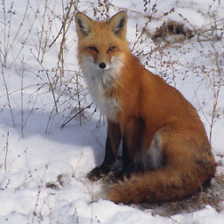
\includegraphics[width=0.085\textwidth]{figures/ptnb_v2/qualitative/butterfly/red_fox_snow/original.png}
        & 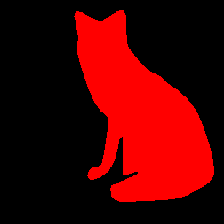
\includegraphics[width=0.085\textwidth]{figures/ptnb_v2/qualitative/butterfly/red_fox_snow/mask.png}
        & 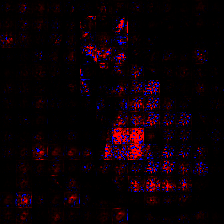
\includegraphics[width=0.085\textwidth]{figures/ptnb_v2/qualitative/butterfly/red_fox_snow/rg_loc.png}
        & 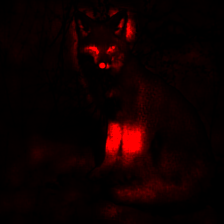
\includegraphics[width=0.085\textwidth]{figures/ptnb_v2/qualitative/butterfly/red_fox_snow/rgeq_loc.png}
        & 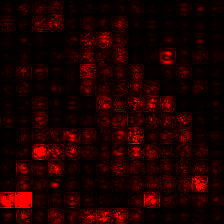
\includegraphics[width=0.085\textwidth]{figures/ptnb_v2/qualitative/butterfly/red_fox_snow/gradient.png}
        & 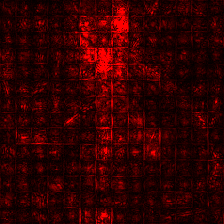
\includegraphics[width=0.085\textwidth]{figures/ptnb_v2/qualitative/butterfly/red_fox_snow/smooth_grad.png}
        & 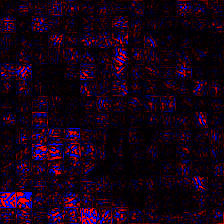
\includegraphics[width=0.085\textwidth]{figures/ptnb_v2/qualitative/butterfly/red_fox_snow/integrated_gradients.png}
        & 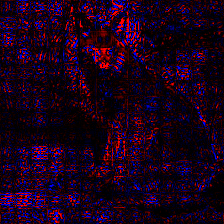
\includegraphics[width=0.085\textwidth]{figures/ptnb_v2/qualitative/butterfly/red_fox_snow/dave.png}
        & 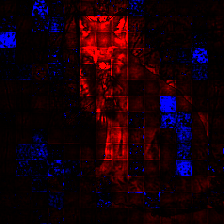
\includegraphics[width=0.085\textwidth]{figures/ptnb_v2/qualitative/butterfly/red_fox_snow/lrp_gamma.png}
        & 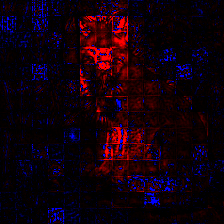
\includegraphics[width=0.085\textwidth]{figures/ptnb_v2/qualitative/butterfly/red_fox_snow/attn_lrp.png}
        & 
\includegraphics[width=0.085\textwidth]{figures/ptnb_v2/qualitative/butterfly/red_fox_snow/tibav.png} \\[1pt]
        \rotatebox{90}{\scriptsize\hspace{6pt}Red fox}
        & 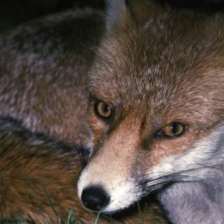
\includegraphics[width=0.085\textwidth]{figures/ptnb_v2/qualitative/butterfly/red_fox/original.png}
        & 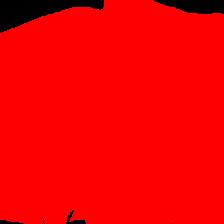
\includegraphics[width=0.085\textwidth]{figures/ptnb_v2/qualitative/butterfly/red_fox/mask.png}
        & 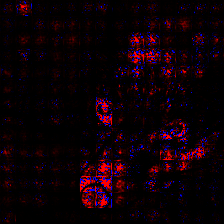
\includegraphics[width=0.085\textwidth]{figures/ptnb_v2/qualitative/butterfly/red_fox/rg_loc.png}
        & 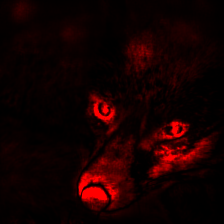
\includegraphics[width=0.085\textwidth]{figures/ptnb_v2/qualitative/butterfly/red_fox/rgeq_loc.png}
        & 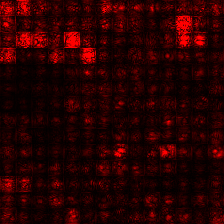
\includegraphics[width=0.085\textwidth]{figures/ptnb_v2/qualitative/butterfly/red_fox/gradient.png}
        & 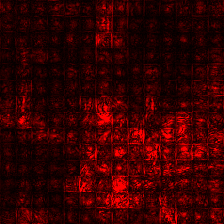
\includegraphics[width=0.085\textwidth]{figures/ptnb_v2/qualitative/butterfly/red_fox/smooth_grad.png}
        & 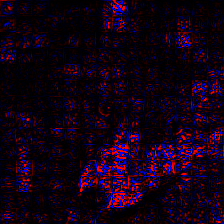
\includegraphics[width=0.085\textwidth]{figures/ptnb_v2/qualitative/butterfly/red_fox/integrated_gradients.png}
        & 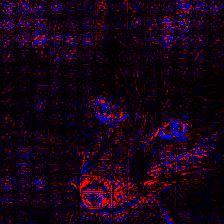
\includegraphics[width=0.085\textwidth]{figures/ptnb_v2/qualitative/butterfly/red_fox/dave.png}
        & 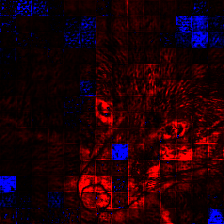
\includegraphics[width=0.085\textwidth]{figures/ptnb_v2/qualitative/butterfly/red_fox/lrp_gamma.png}
        & 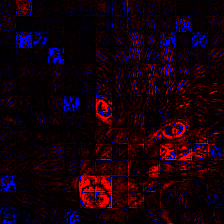
\includegraphics[width=0.085\textwidth]{figures/ptnb_v2/qualitative/butterfly/red_fox/attn_lrp.png}
        & 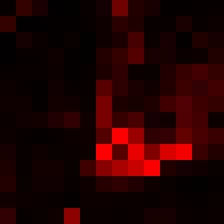
\includegraphics[width=0.085\textwidth]{figures/ptnb_v2/qualitative/butterfly/red_fox/tibav.png} \\[1pt]
        \rotatebox{90}{\scriptsize\hspace{9pt}Kuvasz}
        & 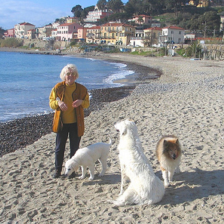
\includegraphics[width=0.085\textwidth]{figures/ptnb_v2/qualitative/butterfly/kuvasz/original.png}
        & 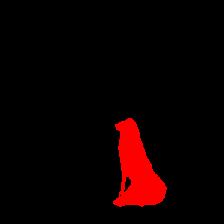
\includegraphics[width=0.085\textwidth]{figures/ptnb_v2/qualitative/butterfly/kuvasz/mask.png}
        & 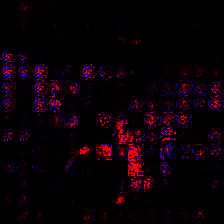
\includegraphics[width=0.085\textwidth]{figures/ptnb_v2/qualitative/butterfly/kuvasz/rg_loc.png}
        & 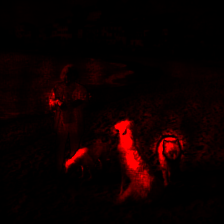
\includegraphics[width=0.085\textwidth]{figures/ptnb_v2/qualitative/butterfly/kuvasz/rgeq_loc.png}
        & 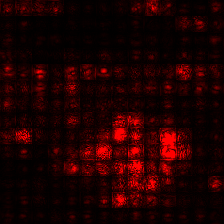
\includegraphics[width=0.085\textwidth]{figures/ptnb_v2/qualitative/butterfly/kuvasz/gradient.png}
        & 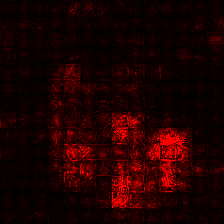
\includegraphics[width=0.085\textwidth]{figures/ptnb_v2/qualitative/butterfly/kuvasz/smooth_grad.png}
        & 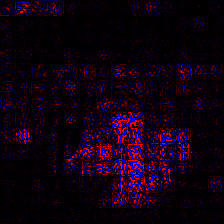
\includegraphics[width=0.085\textwidth]{figures/ptnb_v2/qualitative/butterfly/kuvasz/integrated_gradients.png}
        & 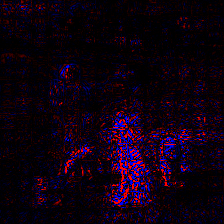
\includegraphics[width=0.085\textwidth]{figures/ptnb_v2/qualitative/butterfly/kuvasz/dave.png}
        & 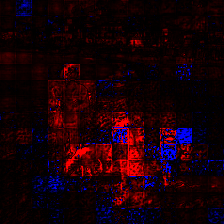
\includegraphics[width=0.085\textwidth]{figures/ptnb_v2/qualitative/butterfly/kuvasz/lrp_gamma.png}
        & 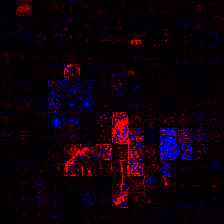
\includegraphics[width=0.085\textwidth]{figures/ptnb_v2/qualitative/butterfly/kuvasz/attn_lrp.png}
        & 
\includegraphics[width=0.085\textwidth]{figures/ptnb_v2/qualitative/butterfly/kuvasz/tibav.png} \\[1pt]
        \rotatebox{90}{\scriptsize\hspace{7pt}Wild boar}
        & 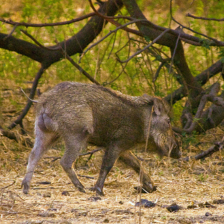
\includegraphics[width=0.085\textwidth]{figures/ptnb_v2/qualitative/butterfly/wild_boar/original.png}
        & 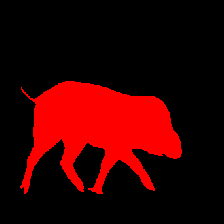
\includegraphics[width=0.085\textwidth]{figures/ptnb_v2/qualitative/butterfly/wild_boar/mask.png}
        & 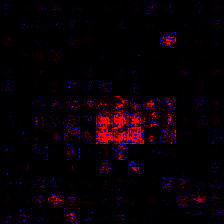
\includegraphics[width=0.085\textwidth]{figures/ptnb_v2/qualitative/butterfly/wild_boar/rg_loc.png}
        & 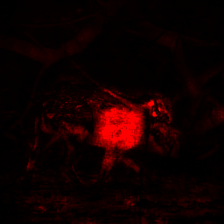
\includegraphics[width=0.085\textwidth]{figures/ptnb_v2/qualitative/butterfly/wild_boar/rgeq_loc.png}
        & 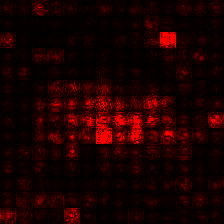
\includegraphics[width=0.085\textwidth]{figures/ptnb_v2/qualitative/butterfly/wild_boar/gradient.png}
        & 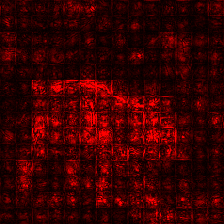
\includegraphics[width=0.085\textwidth]{figures/ptnb_v2/qualitative/butterfly/wild_boar/smooth_grad.png}
        & 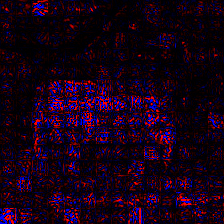
\includegraphics[width=0.085\textwidth]{figures/ptnb_v2/qualitative/butterfly/wild_boar/integrated_gradients.png}
        & 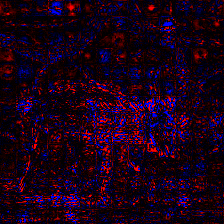
\includegraphics[width=0.085\textwidth]{figures/ptnb_v2/qualitative/butterfly/wild_boar/dave.png}
        & 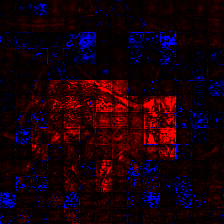
\includegraphics[width=0.085\textwidth]{figures/ptnb_v2/qualitative/butterfly/wild_boar/lrp_gamma.png}
        & 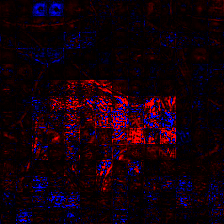
\includegraphics[width=0.085\textwidth]{figures/ptnb_v2/qualitative/butterfly/wild_boar/attn_lrp.png}
        & 
\includegraphics[width=0.085\textwidth]{figures/ptnb_v2/qualitative/butterfly/wild_boar/tibav.png} \\[1pt]
        \rotatebox{90}{\scriptsize\hspace{5pt}Black bear}
        & 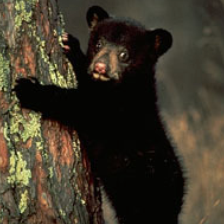
\includegraphics[width=0.085\textwidth]{figures/ptnb_v2/qualitative/butterfly/american_black_bear/original.png}
        & 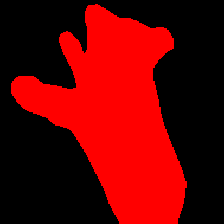
\includegraphics[width=0.085\textwidth]{figures/ptnb_v2/qualitative/butterfly/american_black_bear/mask.png}
        & 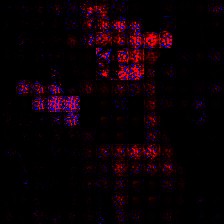
\includegraphics[width=0.085\textwidth]{figures/ptnb_v2/qualitative/butterfly/american_black_bear/rg_loc.png}
        & 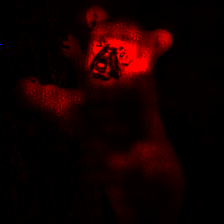
\includegraphics[width=0.085\textwidth]{figures/ptnb_v2/qualitative/butterfly/american_black_bear/rgeq_loc.png}
        & 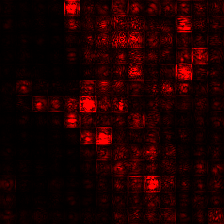
\includegraphics[width=0.085\textwidth]{figures/ptnb_v2/qualitative/butterfly/american_black_bear/gradient.png}
        & 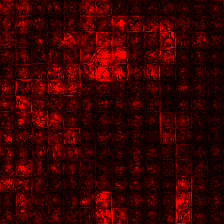
\includegraphics[width=0.085\textwidth]{figures/ptnb_v2/qualitative/butterfly/american_black_bear/smooth_grad.png}
        & 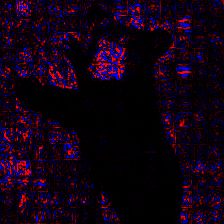
\includegraphics[width=0.085\textwidth]{figures/ptnb_v2/qualitative/butterfly/american_black_bear/integrated_gradients.png}
        & 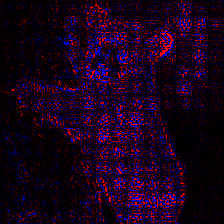
\includegraphics[width=0.085\textwidth]{figures/ptnb_v2/qualitative/butterfly/american_black_bear/dave.png}
        & 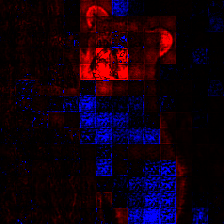
\includegraphics[width=0.085\textwidth]{figures/ptnb_v2/qualitative/butterfly/american_black_bear/lrp_gamma.png}
        & 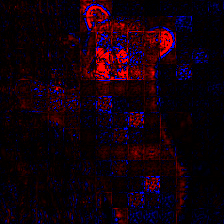
\includegraphics[width=0.085\textwidth]{figures/ptnb_v2/qualitative/butterfly/american_black_bear/attn_lrp.png}
        & 
\includegraphics[width=0.085\textwidth]{figures/ptnb_v2/qualitative/butterfly/american_black_bear/tibav.png} \\[1pt]
        \rotatebox{90}{\scriptsize\hspace{9pt}Airliner}
        & 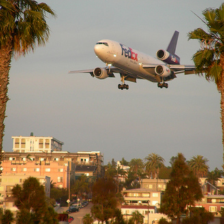
\includegraphics[width=0.085\textwidth]{figures/ptnb_v2/qualitative/butterfly/airliner/original.png}
        & 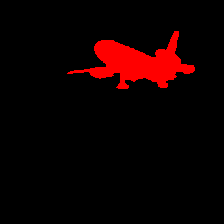
\includegraphics[width=0.085\textwidth]{figures/ptnb_v2/qualitative/butterfly/airliner/mask.png}
        & 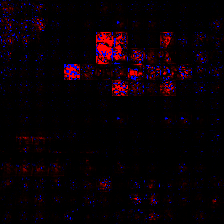
\includegraphics[width=0.085\textwidth]{figures/ptnb_v2/qualitative/butterfly/airliner/rg_loc.png}
        & 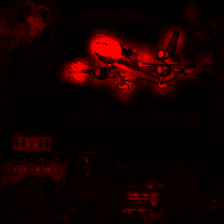
\includegraphics[width=0.085\textwidth]{figures/ptnb_v2/qualitative/butterfly/airliner/rgeq_loc.png}
        & 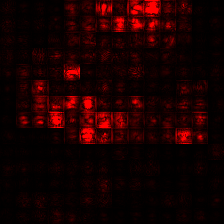
\includegraphics[width=0.085\textwidth]{figures/ptnb_v2/qualitative/butterfly/airliner/gradient.png}
        & 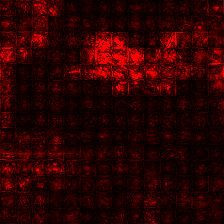
\includegraphics[width=0.085\textwidth]{figures/ptnb_v2/qualitative/butterfly/airliner/smooth_grad.png}
        & 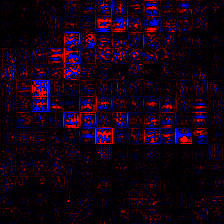
\includegraphics[width=0.085\textwidth]{figures/ptnb_v2/qualitative/butterfly/airliner/integrated_gradients.png}
        & 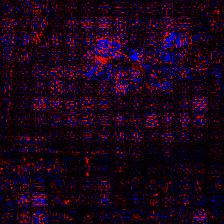
\includegraphics[width=0.085\textwidth]{figures/ptnb_v2/qualitative/butterfly/airliner/dave.png}
        & 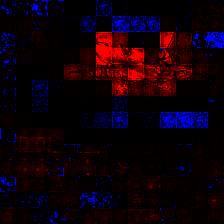
\includegraphics[width=0.085\textwidth]{figures/ptnb_v2/qualitative/butterfly/airliner/lrp_gamma.png}
        & 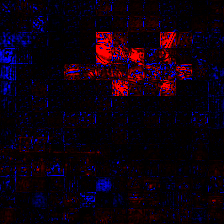
\includegraphics[width=0.085\textwidth]{figures/ptnb_v2/qualitative/butterfly/airliner/attn_lrp.png}
        & 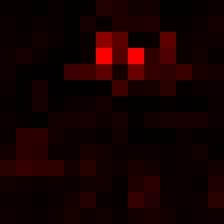
\includegraphics[width=0.085\textwidth]{figures/ptnb_v2/qualitative/butterfly/airliner/tibav.png} \\
    \end{tabular}
    }
    }%
\caption[ViT-B/16 qualitative comparison on six ImageNet-S examples]{Six ImageNet-S examples, ViT-B/16, at the configurations specified above. Red and blue show positive and negative attribution. Each sign is divided by its image-wide 99th percentile and clipped, saturating the top 1\% so concentrated maps remain legible; every method uses this display transform.}
    \label{ptnb:fig:qualitative}
\end{figure}
\par\medskip
